
\chapter{Resultados}
Nessa seção apresentamos os principais resultados na elaboração desse trabalho. Eles são referentes a análise da base de dados, função de custo, autocodificador esparso e alocação dinâmica de bits. 
%A nossa hipótese é que a performance do autoencoder está relacionado com características da entropia da base de dados utilizado no treinamento.
Treinamos 5 modelos do autocodificador para cada base de dados apresentada em \ref{list:bds} e usando a função MAE sobre os resíduos como função de custo. Além disso, os seguintes hiper-parâmetros da rede foram adotados nesse experimento: 

\begin{enumerate}
	\label{enum:hiper_param}
	\item Tamanho do lote: 32; 
	\item Número de lotes de treinamento por época: 38 mil (aproximadamente);   
	\item Número de iterações: 16;
	\item Número de épocas: 1;
	\item Otimizador: Adam;
	\item Taxa de aprendizado: $5 \times {10}^{-4}$
\end{enumerate}

Calculamos os valores médios de PSNR, SSIM e MS-SSIM das imagens da Kodak reconstruídas na taxa nominal de 2 bits por pixel. Os resultados estão disponíveis na tabela \ref{table:comp_datasets}.


\begin{table}[htbp]
	\centering
	\caption{Comparação das base de dados.}
	\begin{tabular}{|l|l|l|l|}
		\hline
		\textbf{Base de dados} & \textbf{PSNR(dB)}    & \textbf{SSIM}   & \textbf{MS-SSIM}\\\hline
		\textbf{0}            & 25,4268          & 0,6978          & 0,9177           \\\hline
		\textbf{1}            & 31,9458          & 0,9201          & 0,9874           \\\hline
		\textbf{2}            & 34,3622          & 0,9444          & 0,9900           \\\hline
		\textbf{3}            & 32,9632	       & 0,9327          & 0,9890           \\\hline
		\textbf{4}            & \textbf{34,3903} & \textbf{0,9473} & \textbf{0,9913}     
		\\ \hline
	\end{tabular}
	\label{table:comp_datasets}
\end{table}

Conforme esperado, uma base de dados de alta entropia é indicada para melhorar a performance do modelo. A hipótese é que essa característica otimiza a rede a aprender padrões não triviais das imagens e evitar o sobre-ajuste do modelo. A base de dados 4, nessa tabela, obteve o melhor resultado por uma margem pequena em relação a BD2. 
Para temos uma comparação mais ampla, calculamos as áreas abaixo das curvas de PSNR $\times$ taxa, SSIM $\times$ taxa e  MS-SSIM $\times$ taxa dos modelos treinados por DB2 e DB4. Em todas as curvas temos 16 pontos com taxas nominais no intervalo de 0,125 a 2,0 bpp com incrementos constantes de 0,125 bpp. A Figura \ref{fig:auc1} é mais um indicativo que o modelo treinado pela BD4 apresenta a melhor performance.    


Por esse motivo, calculamos a área abaixo da curva   

\begin{figure}
	\centering
	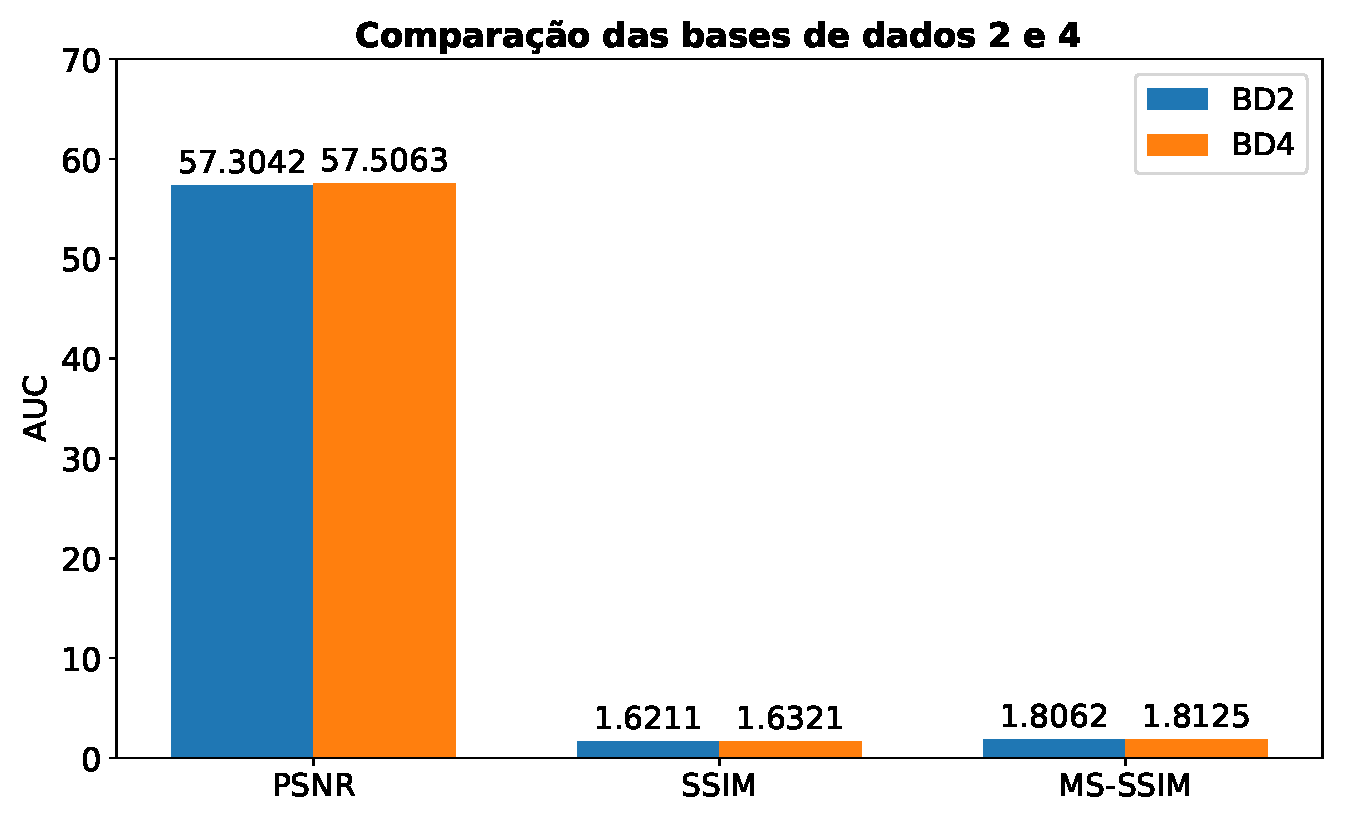
\includegraphics[width=0.7\textwidth]{figuras/auc1.pdf}
	\caption[Comparação das bases de dados pela área abaixo das curvas em métricas de qualidade]{Essa Figura mostra as áreas abaixo da curvas de PSNR, SSIM e MS-SSIM cada uma em função das taxas nominais do modelo com 16 iterações.}
	\label{fig:auc1}
\end{figure}

A BD4 obteve os melhores resultados nas 3 métricas nesse conjunto de teste e será aplicada nas próximas análises.

O próximo passo foi analisar a performance no modelo à medida que aumentarmos o número de épocas de treinamento.
Para isso, treinamos o modelo por 13 épocas usando somente a base de dados 4. Os parâmetros do novo treinamento foram definido conforme itens citados em \ref{enum:hiper_param}, exceto o número de épocas. A evolução do modelo ao passar das época pode ser vista na Figura \ref{fig:psnr_13epocas}. 

\begin{figure}
	\centering
	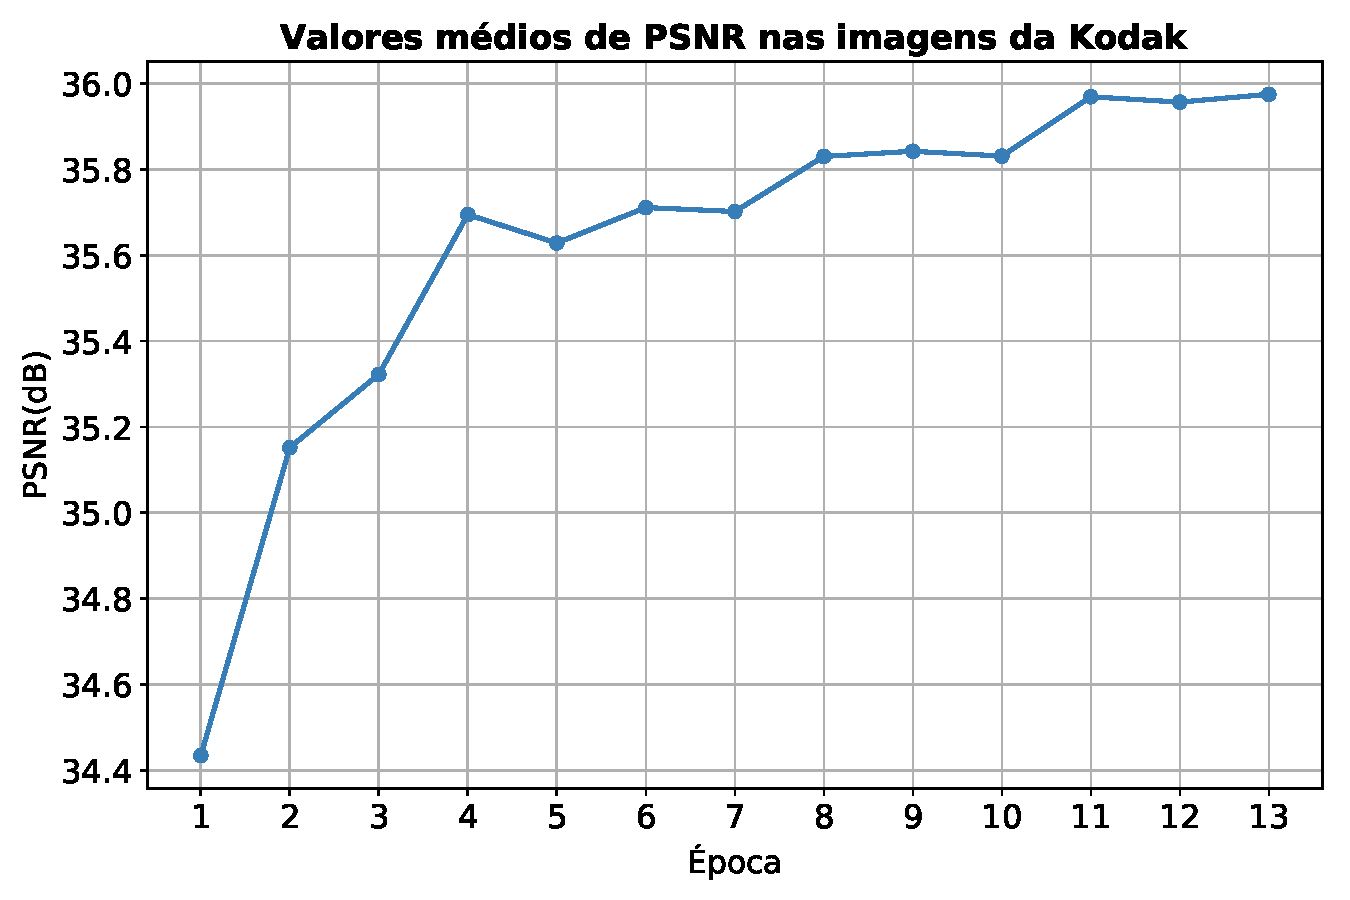
\includegraphics[width=0.9\textwidth]{figuras/psnr_13epochs.pdf}
	\caption[Performance do modelo em função do número de épocas de treinamento]{Performance do modelo em função do número de épocas de treinamento. Para cada época, calculamos a PSNR média das imagens da Kodak reconstruídas com taxa de 2 bpp.  O ganho de desempenho do autocodificador entre a primeira e 13ª época foi de um pouco mais que 1,5dB.}
	\label{fig:psnr_13epocas}
\end{figure}		

Usando o modelo obtido na 13ª época, plotamos as curvas de distorção nas métricas SSIM e MS-SSIM em conjunto com o JPEG(4:2:0) e o trabalho de Toderici et. al. \cite{FullResolution2017Toderici}. Essas Figuras estão disponíveis em \ref{fig:ssim_ae_jpeg_toderici} e   \ref{fig:msssim_ae_jpeg_toderici}. 
Observamos que nessas métricas e na média das imagens da Kodak, o nosso modelo supera o trabalho de Toderici et. al. e o JPEG. Acreditamos que esse resultado se deve a escolha criteriosa da base de dados de treinamento que não passaram por processos de compressão com perdas e decimação.

\begin{figure}
	\centering
	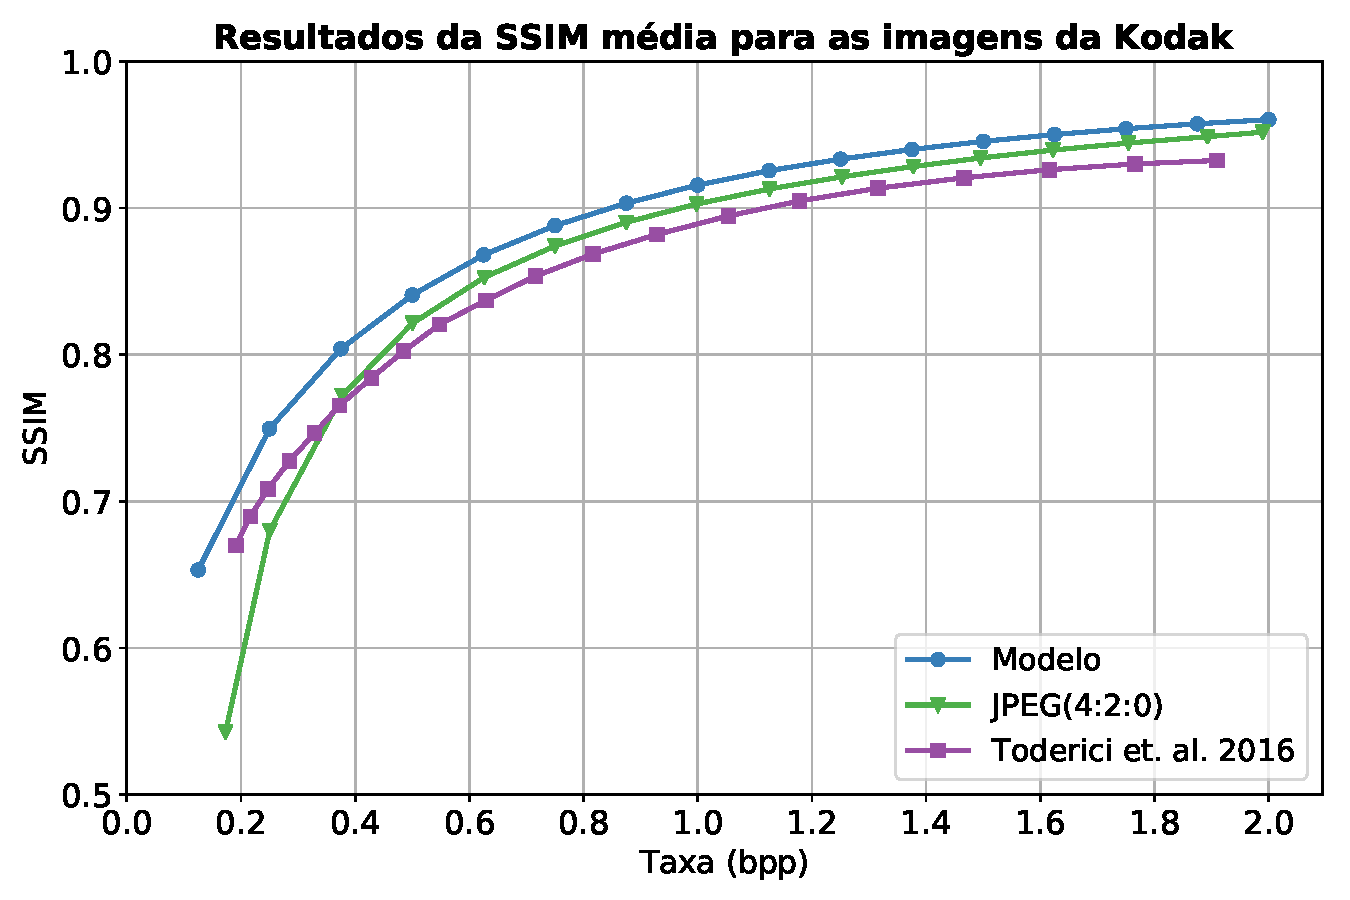
\includegraphics[width=0.9\textwidth]{figuras/ssim_ae_jpeg_toderici.pdf}
	\caption{Comparação.}
	\label{fig:ssim_ae_jpeg_toderici}
\end{figure}	



\begin{figure}
	\centering
	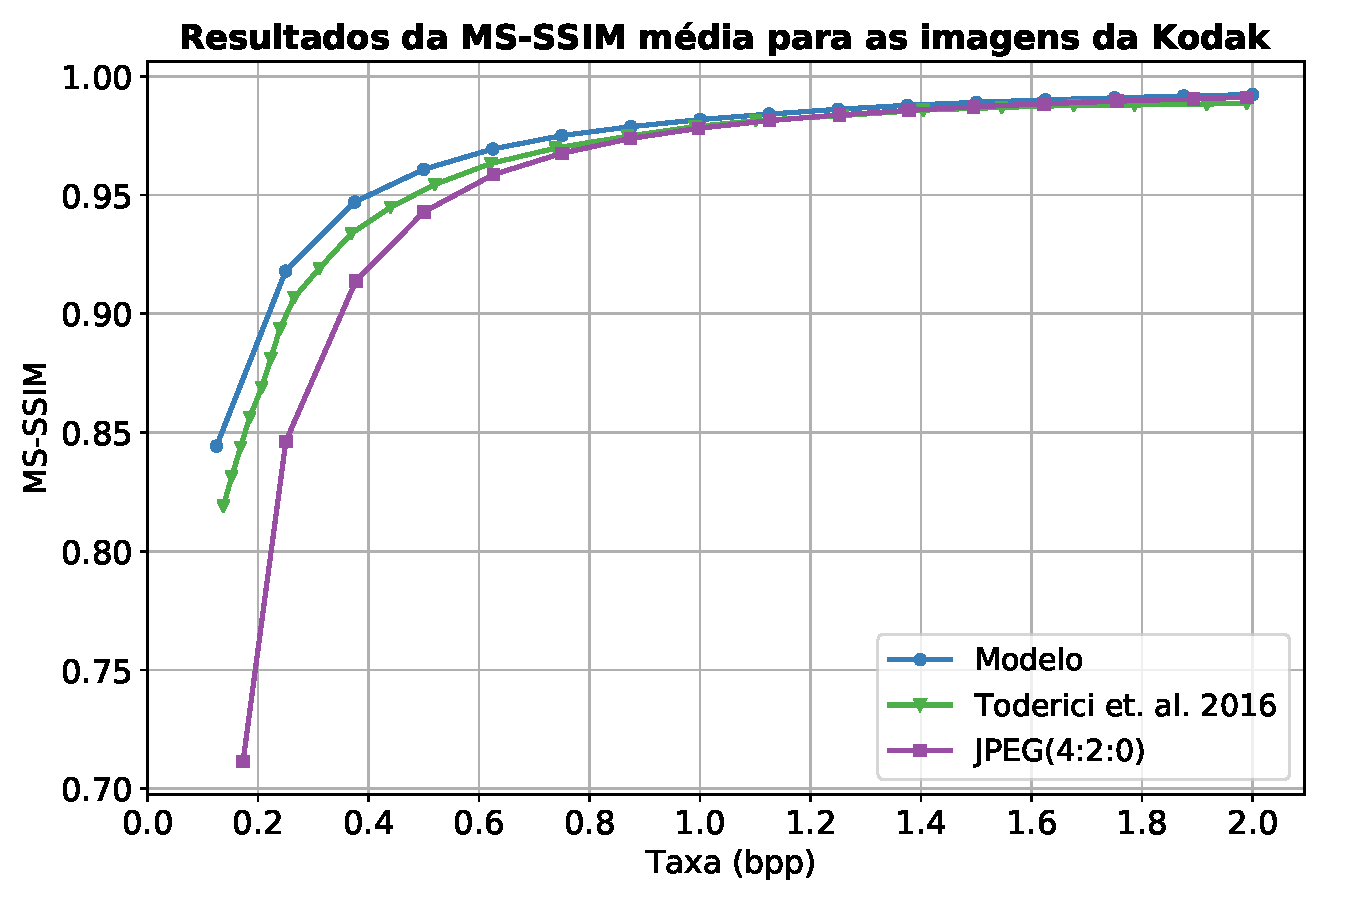
\includegraphics[width=0.9\textwidth]{figuras/msssim_ae_jpeg_toderici.pdf}
	\caption{Comparação.}
	\label{fig:msssim_ae_jpeg_toderici}
\end{figure}	


Todavia, a Figura \ref{fig:psnr_ae_jpeg} indica que na métrica PSNR o JPEG(4:2:0) ainda supera o nosso modelo para a maioria das taxas calculadas. 

\begin{figure}
	\centering
	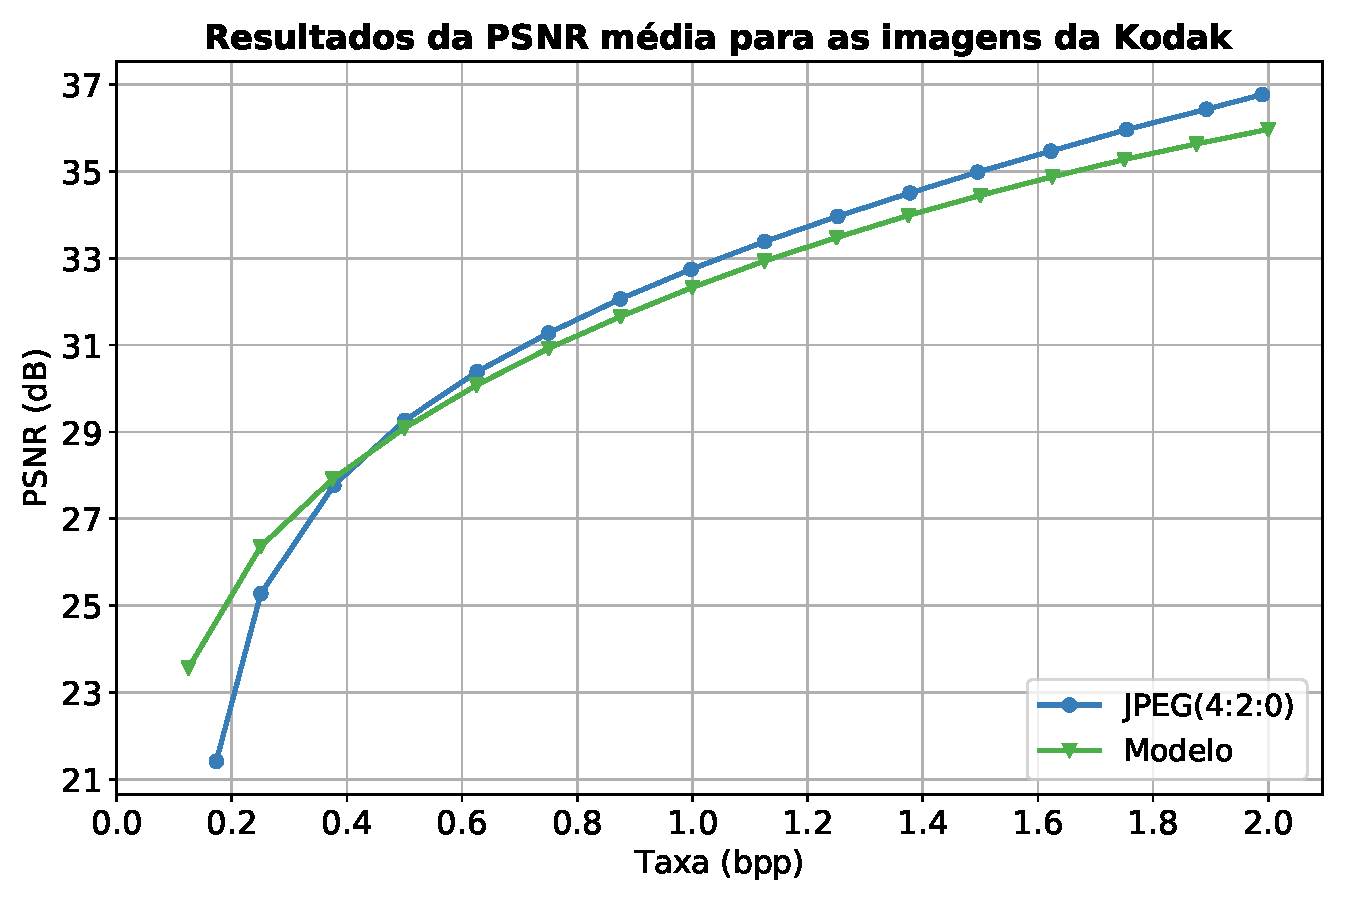
\includegraphics[width=0.9\textwidth]{figuras/psnr_ae_jpeg.pdf}
	\caption{Comparação.}
	\label{fig:psnr_ae_jpeg}
\end{figure}	


Pela figura \ref{fig:psnr_13epocas} verificamos uma tendência de saturação do modelo, em torno de 36 dB na taxa de 2 bpp, ao passar da épocas de treinamento. Dessa forma, exploraremos novas técnicas que podem gerar menores taxas de compressão sem impactar na qualidade das imagens reconstruídas pelo decodificador.


%A função de custo é outra escolha importante nos treinamento de RNA. No problema de compressão de imagens a escolha dessa função tem o agravante de não haver consenso entre os pesquisadores de uma métrica ideal para avaliar a qualidade entre uma imagem original e a sua versão reconstruída.  Na hipótese de haver tal função, poderíamos definir uma função de erro em relação a métrica ideal como função de custo e minimizar o seu valor ao longo do aprendizado do modelo. 
%Contudo, algumas funções apresentam relações da medida de distorção entre uma imagem e sua reconstrução, tais como MSE, MAE, 1-SSIM, 1-MS-SSIM, etc. Vamos definir algumas variações dessas funções. 


%\begin{equation}
%	\begin{aligned}
%    \centering    
%      MAE(X,X') = \displaystyle\frac{1}{n}\sum_{t=1}^{n}\left\|X_{t} - X'_{t}\right\|
%	\end{aligned}
%\end{equation}




A Tabela \ref{table:comp_loss} apresenta resultados para 7 funções de custo que mensuram a distorção entre duas imagens.  Os valores foram calculados pela média das imagens da Kodak codificadas a 2 bpp. A rede foi treinada com a base de dados 4 e parâmetros listados em	\ref{enum:hiper_param}. Nessa tabela, $R$, $R'$, $X$ e $X'$ foram definidos na Equação \ref{eq:model_1it}, omitindo-se a dependência temporal. A medida $X-X'$ é o resíduo em relação a imagem como um todo, onde $X$ é fixo.  
O subíndice \textit{y} e \textit{$C_bC_r$} são para indicar a componente de luminância e o par crominância azul e vermelho, respectivamente. Nos testes 3 e 4, modificamos o treinamento para rede operar no espaço $YC_bC_r$. O objetivo foi penalizar, predominante, o erro da componente de luminância (que contém informações mais sensíveis ao olho humano) no ajuste da rede, em comparação com as componentes de crominância.
No teste 7, utilizamos uma medida de dissimilaridade estrutural entre duas imagens, obtida a partir da SSIM e implementada em \cite{su2017}.  A distorção calculada pela MSE forneceu os melhores resultados em todas as métricas avaliadas. 


\begin{table}[]
	\centering
	\caption{Comparação das funções de custo.}
	\begin{adjustbox}{width=\columnwidth,center}	
	\begin{tabular}{|l|l|l|l|l|l|l|}
		\hline
		\textbf{Teste} & \textbf{Função de custo}                                                                                        & \textbf{Espaco} & \textbf{PNSR (dB)} & \textbf{PNSR Y (dB)} & \textbf{SSIM}   & \textbf{MS-SIM} \\ \hline
		\textbf{1}     & $MAE(R-R’)$                                                                                                     & RGB             & 33,0872            & 33,8443              & 0,9309          & 0,9876          \\ \hline
		\textbf{2}     & $MAE^{2}(R-R’)$                                                                                                 & RGB             & 34,1766            & 34,9706              & 0,9444          & 0,9892          \\ \hline
		\textbf{3}     & \begin{tabular}[c]{@{}l@{}}$MAE^{2}(R_{y}-R_{y}’) +$\\ $+ 0.25 \times MAE^{2}(R_{CbCr}-R_{CbCr}’)$\end{tabular} & YCbCr           & 33,3555            & 35,3253              & 0,9445          & 0,9857          \\ \hline
		\textbf{4}     & \begin{tabular}[c]{@{}l@{}}$MSE(R_{y}-R_{y}’) +$\\ $+ 0.25 \times MSE(R_{CbCr}-R_{CbCr}’)$\end{tabular}         & YCbCr           & 33,5249            & 35,1863              & 0,9390          & 0,9858          \\ \hline
		\textbf{5}     & $MSE(R-R’)$                                                                                                     & RGB             & \textbf{34,9259}   & \textbf{35,9066}     & \textbf{0,9474} & \textbf{0,9907} \\ \hline
		\textbf{6}     & $MSE(X-X’)$                                                                                                     & RGB             & 33,7662            & 34,6014              & 0,9321          & 0,9866          \\ \hline
		\textbf{7}     & $1 - SSIM (X -X’)$                                                                                              & RGB             & 33,2754            & 34,0755              & 0,9352          & 0,9896          \\ \hline
	\end{tabular}
	\end{adjustbox}
	\label{table:comp_loss}
\end{table}

A segunda etapa na escolha de uma função de perdas foi considerar, de forma implícita, a taxa ao aplicar a função \ref{eq:rdo} com um $\lambda(t)$ obtida de forma experimental e dado por: 

\begin{equation}
\lambda(t) = 3,5 \times 10^{-7} \times e^{-0,01 \times (t+1)}  
\end{equation}

Além dessa modificação, usamos a base de dados 5 obtida conforme a regra da base de dados 4 sem a aleatoriedade no sorteio dos blocos de alta entropia e alterações o número de estágios de treinamento de 16 para 28. O aumento no número de estágios de treinamento visa permitir melhores reconstruções das imagens pelo codificador. Desejamos que o aumento da taxa nominal seja compensada pela codificação com o GZIP.  Resumindo, no novo treinamento da rede teremos: 

\begin{enumerate}
	\label{enum:hiper_param2}
	\item Tamanho do lote: 32;  
	\item Número de lotes de treinamento por época: 71 mil (aproximadamente);   
	\item Número de iterações no treinamento: 28;
	\item Número de iterações durante os testes: 22;
	\item Número de épocas: 27;
	\item Otimizador: Adam;
	\item Taxa de aprendizado: $5 \times {10}^{-4}$ com decaimento por um fator de 0,5 caso a média da função de perdas em uma época seja maior que na época anterior.
\end{enumerate}
A Figura \ref{fig:gain_gzip_meida} compara o ganho proporcionado pela codificação de entropia do GZIP ao plotarmos as curvas de PNSR (a) e SSIM (b) em função da taxa usando as imagens da Kodak. Ao usarmos a taxa real as curvas se deslocam para esquerda. Observamos, que o ganho do GZIP é maior em taxas maiores. Isso é esperado tendo em vista que, em geral, os codificadores de entropia são mais eficientes em conjuntos maiores de dados. Nos próximos testes, as taxas empregadas serão sempre a real.    

\begin{figure}
	\centering
	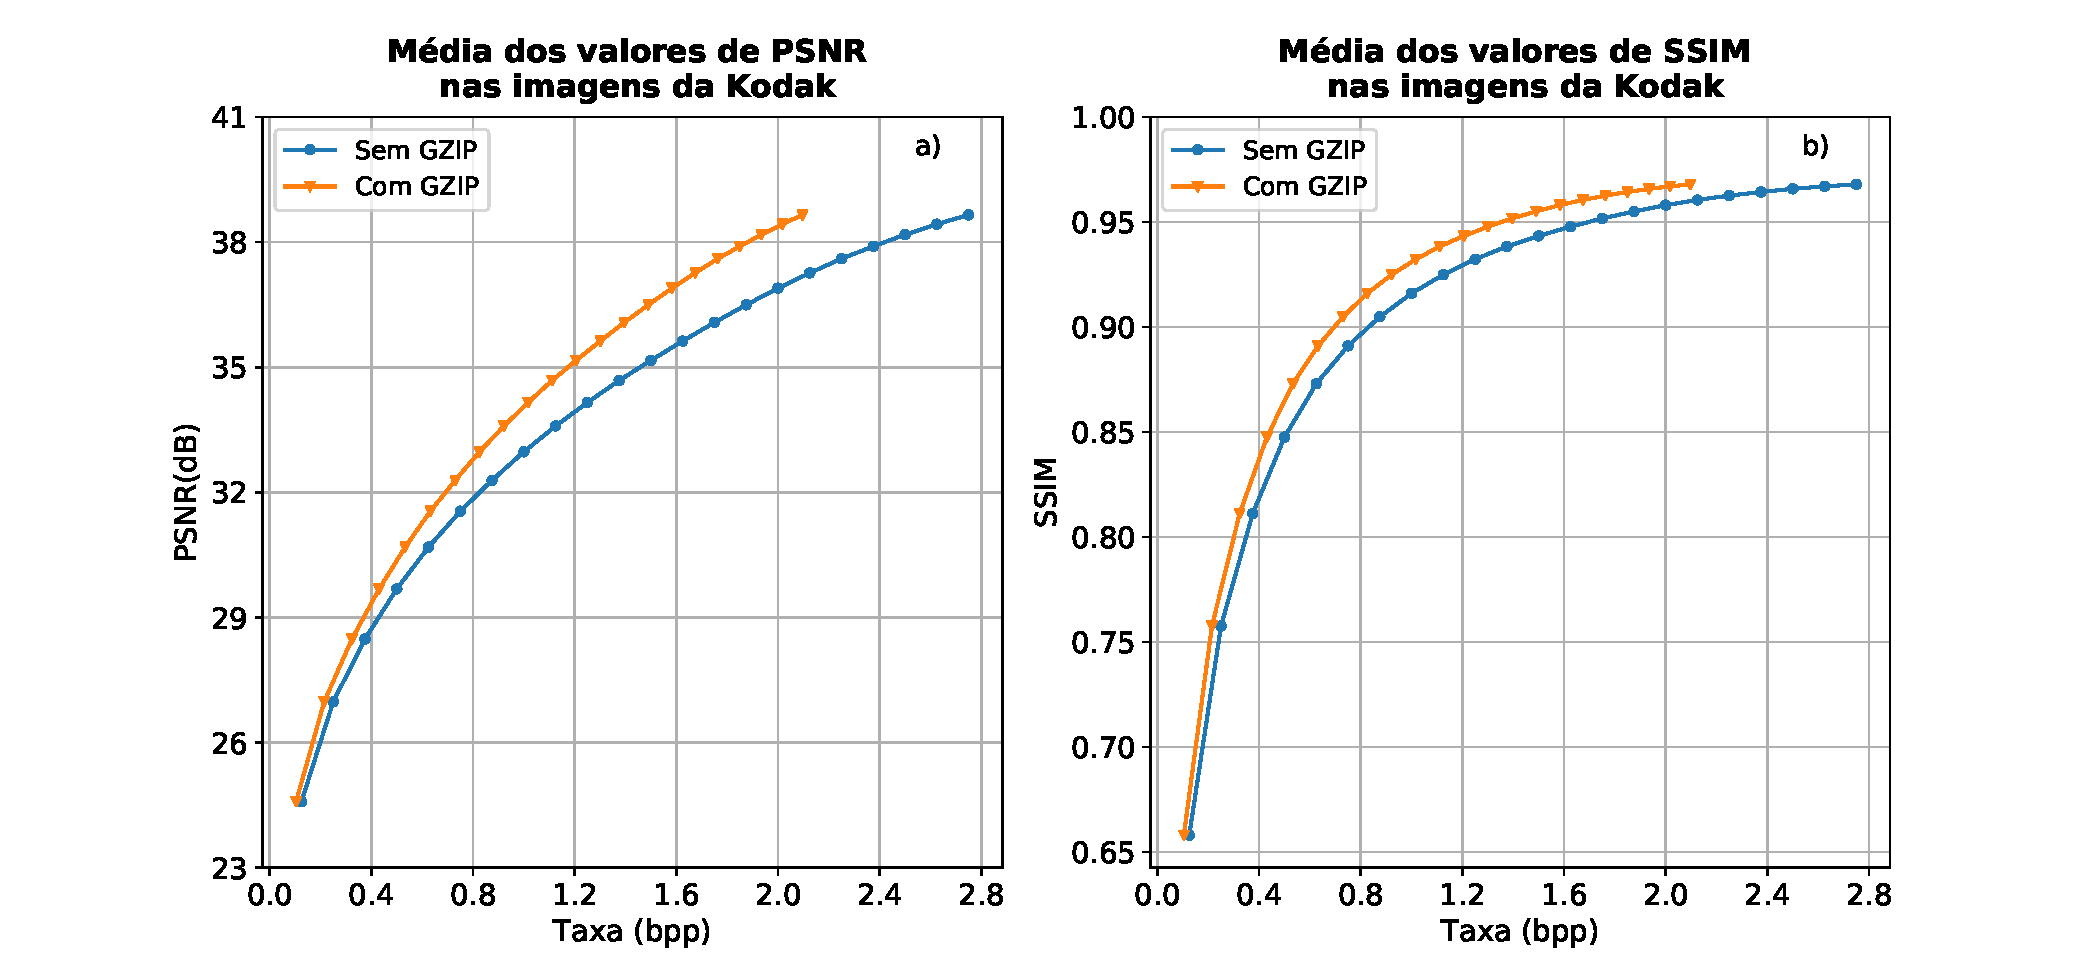
\includegraphics[width=1.1\textwidth]{figuras/gain_gzip_media.pdf}
	\caption[Comparação de codificação com e sem o GZIP]{Nessa figura, ilustramos o resultado em aplicar o GZIP na sequência binária gerada no codificador. As curvas foram plotadas usando o modelo treinado até a época 26.}  	
	\label{fig:gain_gzip_meida}
\end{figure}

A Figura \ref{fig:taxa_bd} mostra como a performance em termos de taxa-BD (em relação ao jPEG) se comporta durante o treinado do modelo. O treinamento em várias épocas melhora significativamente o desempenho do modelo. É verdade também que a taxa com que o modelo apresenta melhores resultados se torna mais lenta ao passar das épocas. A economia da taxa na última época em relação a primeira é aproximadamente de 17\%. Nesse teste, a 26ª época gerou o modelo de melhor desempenho.  



\begin{figure}
	\centering
	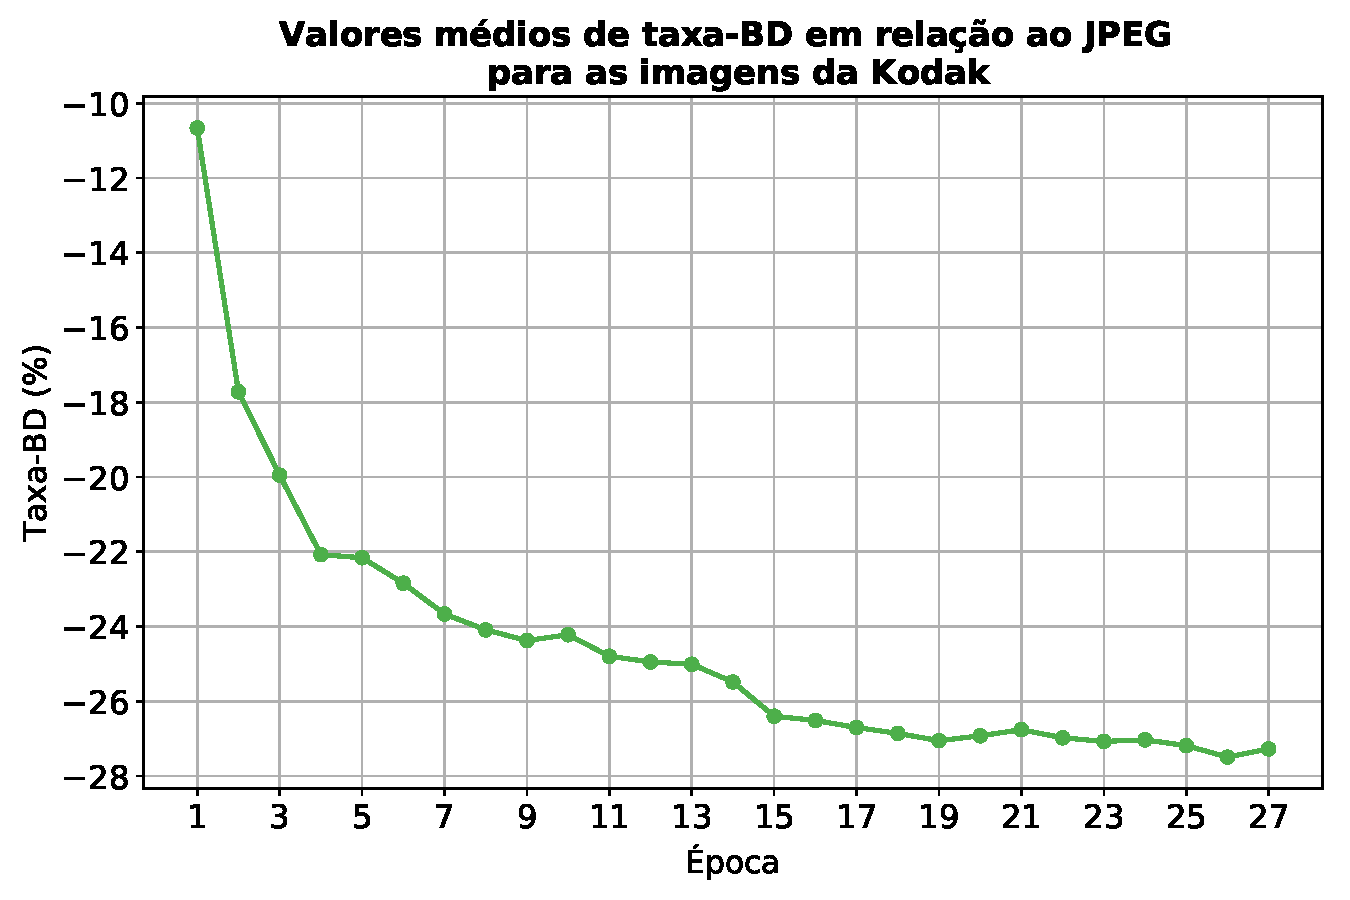
\includegraphics[width=1\textwidth]{figuras/taxa_bd_27epocas.pdf}
	\caption{Ilustração da porcentagem da taxa-BD média sobre a base de dados da Kodak e tendo o JPEG como âncora.  Valores cada vez mais negativos indicam que a economia média de taxa de bits do nosso modelo em relação ao JPEG aumenta para uma dada qualidade equivalente de PSNR na média das imagens da Kodak.}  
	\label{fig:taxa_bd}
\end{figure}	

Nas figuras em \ref{fig:metricas_3ep} podemos observar a otimização taxa-distorção em 3 épocas. Nesse teste, a qualidade melhora e a taxa real é reduzida seguindo a época 1, 6 e 26. A qualidade aqui é modelada pelas curvas de PSNR (a), PSNR Y (b)  SSIM (c) e  MS-SSIM (d). Esse resultado indica que a nossa função consegue alcançar as hipóteses apresentadas, contudo não temos uma fundamentação na direção do melhor método para otimizar taxa-distorção.  

\begin{figure}
	\centering
	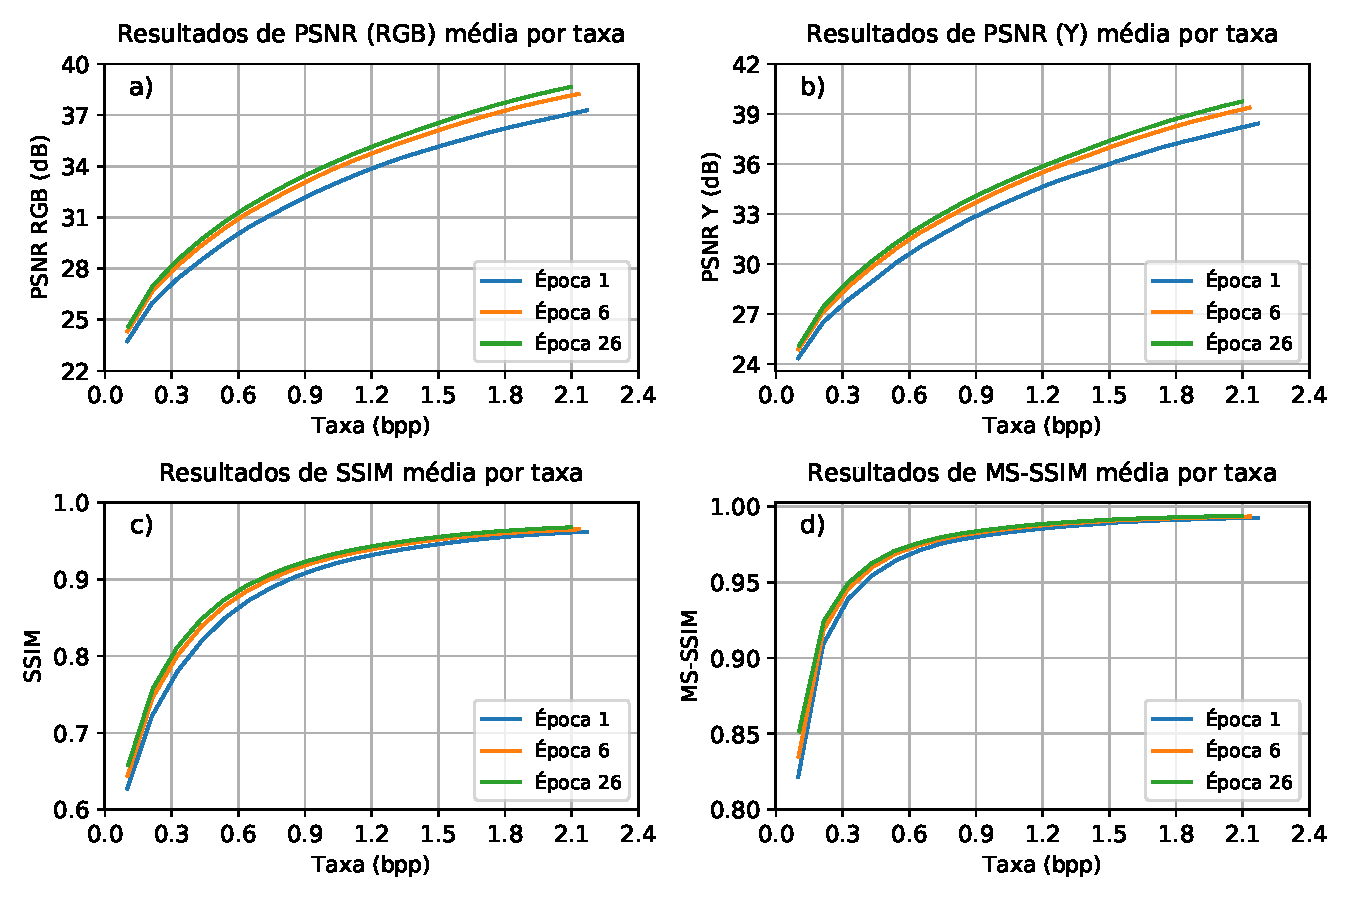
\includegraphics[width=1\textwidth]{figuras/result_3ep.pdf}
	\caption[Curvas de qualidade por taxa em 3 épocas distintas]{Figuras mostrando a evolução do modelo em termos de taxa e 4 métricas de qualidade em 3 épocas distintas. Nas 4 curvas taxa e distorção apresentam melhores resultado no passar da primeira, sexta e vigésima-sexta épocas}  	
	\label{fig:metricas_3ep}
\end{figure}

A Figura \ref{fig:gain_medio_bpp} apresenta o ganho médio percentual da taxa real (fornecida pelo GZIP) em relação a nominal como função da iteração em que as imagens foram reconstruídas. Os resultados mostram que, aproximadamente, nos primeiros 3 níveis de reconstrução o modelo final tem ganho médio menor em relação a primeira e sexta versão do modelo. Além disso, nesses 3 níveis o ganho é reduzido ainda que temos um conjunto maior de bits para realizar compressão.  
A justificativa pode ser que, durante o treinamento, para esse nível de reconstrução a função da distorção é significativamente superior ao valor da função que modela a taxa aproximadamente. Então, ao priorizar a reconstrução a proporção de zeros e uns é condicionada para reduzir a distorção. Esse fato não garante que a entropia de ordem 0 do fluxo de bits seja baixa. Além isso, o fator de regularização influencia de forma indireta na distorção.
A partir da 4ª iteração a curva de ganho do modelo final ultrapassa as demais. Á medida que a reconstrução é feita, esperamos que em um momento a relevância da distorção no aprendizagem da rede seja reduzida e a entropia de ordem 0 dos bits seja otimizada. 



\begin{figure}
	\centering
	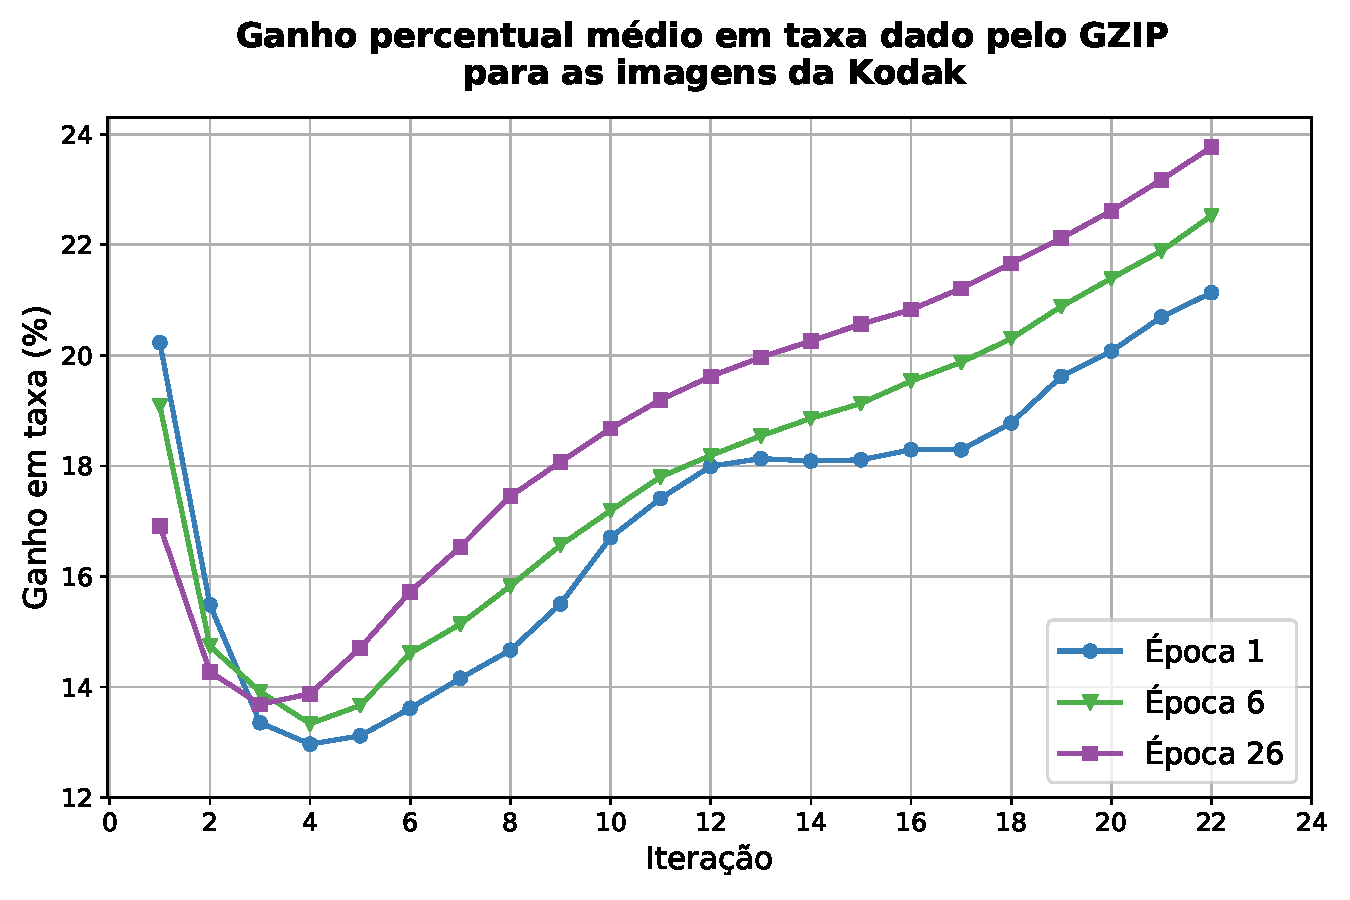
\includegraphics[width=0.9\textwidth]{figuras/ganho_taxa_3epocas.pdf}
	\caption[Ganho do GZIP por nível de reconstrução]{Figura com o ganho do GZIP por nível de reconstrução e na média para as 24 imagens da Kodak em 3 codecs. De forma geral, nas primeiras iterações ocorre redução no ganho e a partir da quarta iteração o ganho de taxa é crescente.}  	
	\label{fig:gain_medio_bpp}
\end{figure}


%\begin{figure}
%	\centering
%	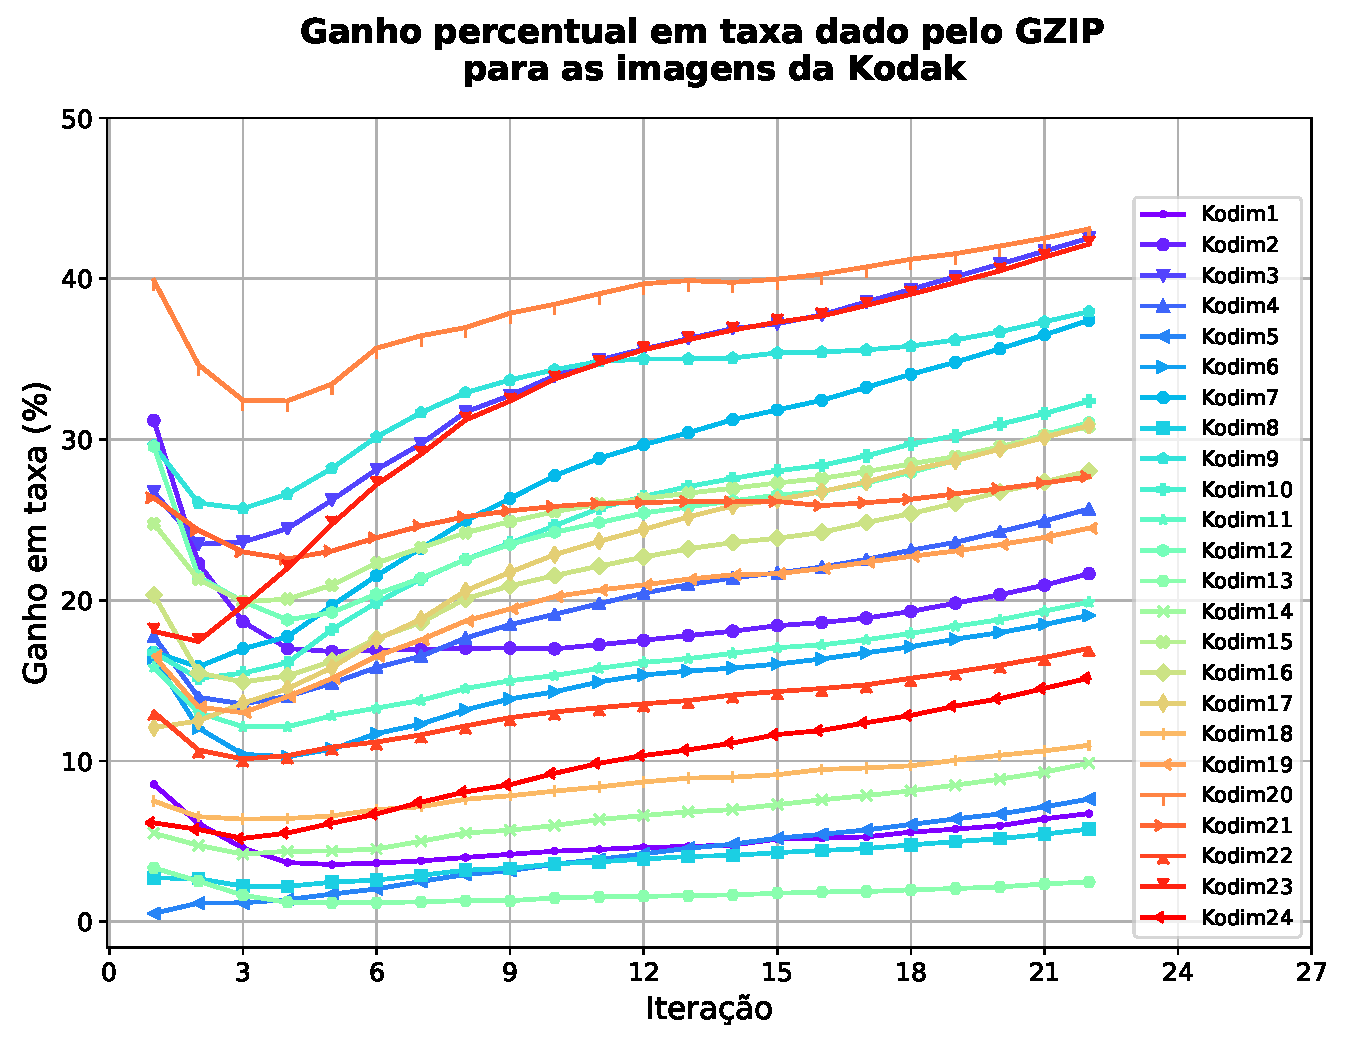
\includegraphics[width=1.0\textwidth]{figuras/ganho_taxa_kodak_epoca26.pdf}
%	\caption{}  	
%	\label{fig:gain_bpp}
%\end{figure}

%\begin{figure}
%	\centering
%	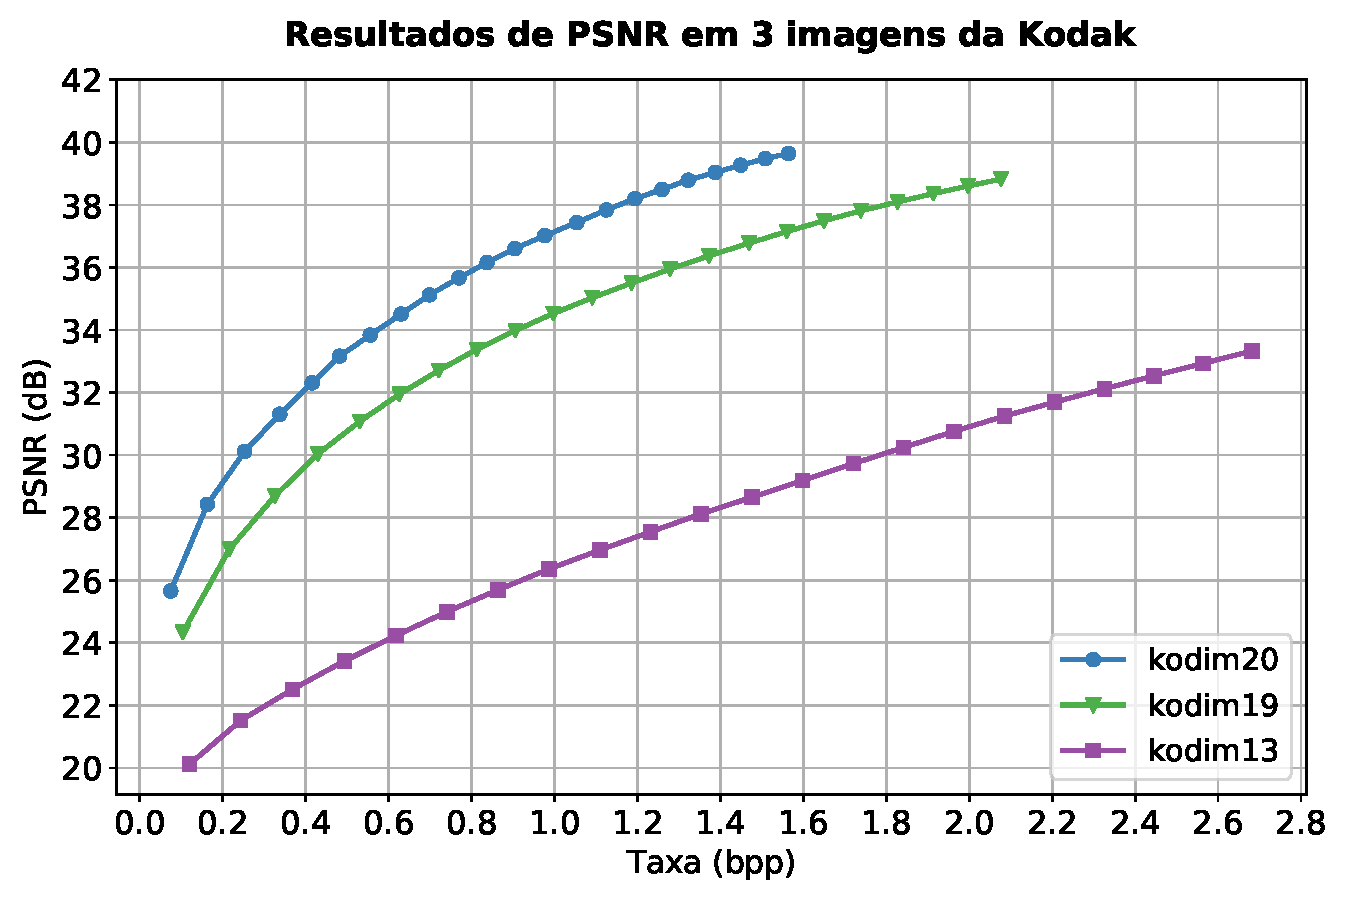
\includegraphics[width=0.9\textwidth]{figuras/rdo_3examples.pdf}
%	\caption{}  	
%	\label{fig:rdo_3examples}
%\end{figure}
Nas Figuras \ref{comp_gain_psnr} selecionamos 3 imagens para plotar as curvas de PSNR e ganho. Do nosso conjunto de teste, a koddim13  apresenta o menor ganho, a kodim20 tem o maior ganho e a kodim6 tem ganho aproximadamente próximo da média. 
Nesse teste, a kodim20 apresenta a maior qualidade (ou menor distorção) dentre os exemplos. Supomos que a rede conseguiu capturar ou ``aprender'' padrões com a semântica espacial presente na kodim20 com uma representação latente esparsa. 
Em contrapartida, acreditamos a imagem kodim13 contém muita informação de alta frequência e de ``difícil compressão''. Essas imagens com suas reconstruções estão disponíveis ns Figura \ref{fig:kodim13}.   


\begin{figure}
	\centering
	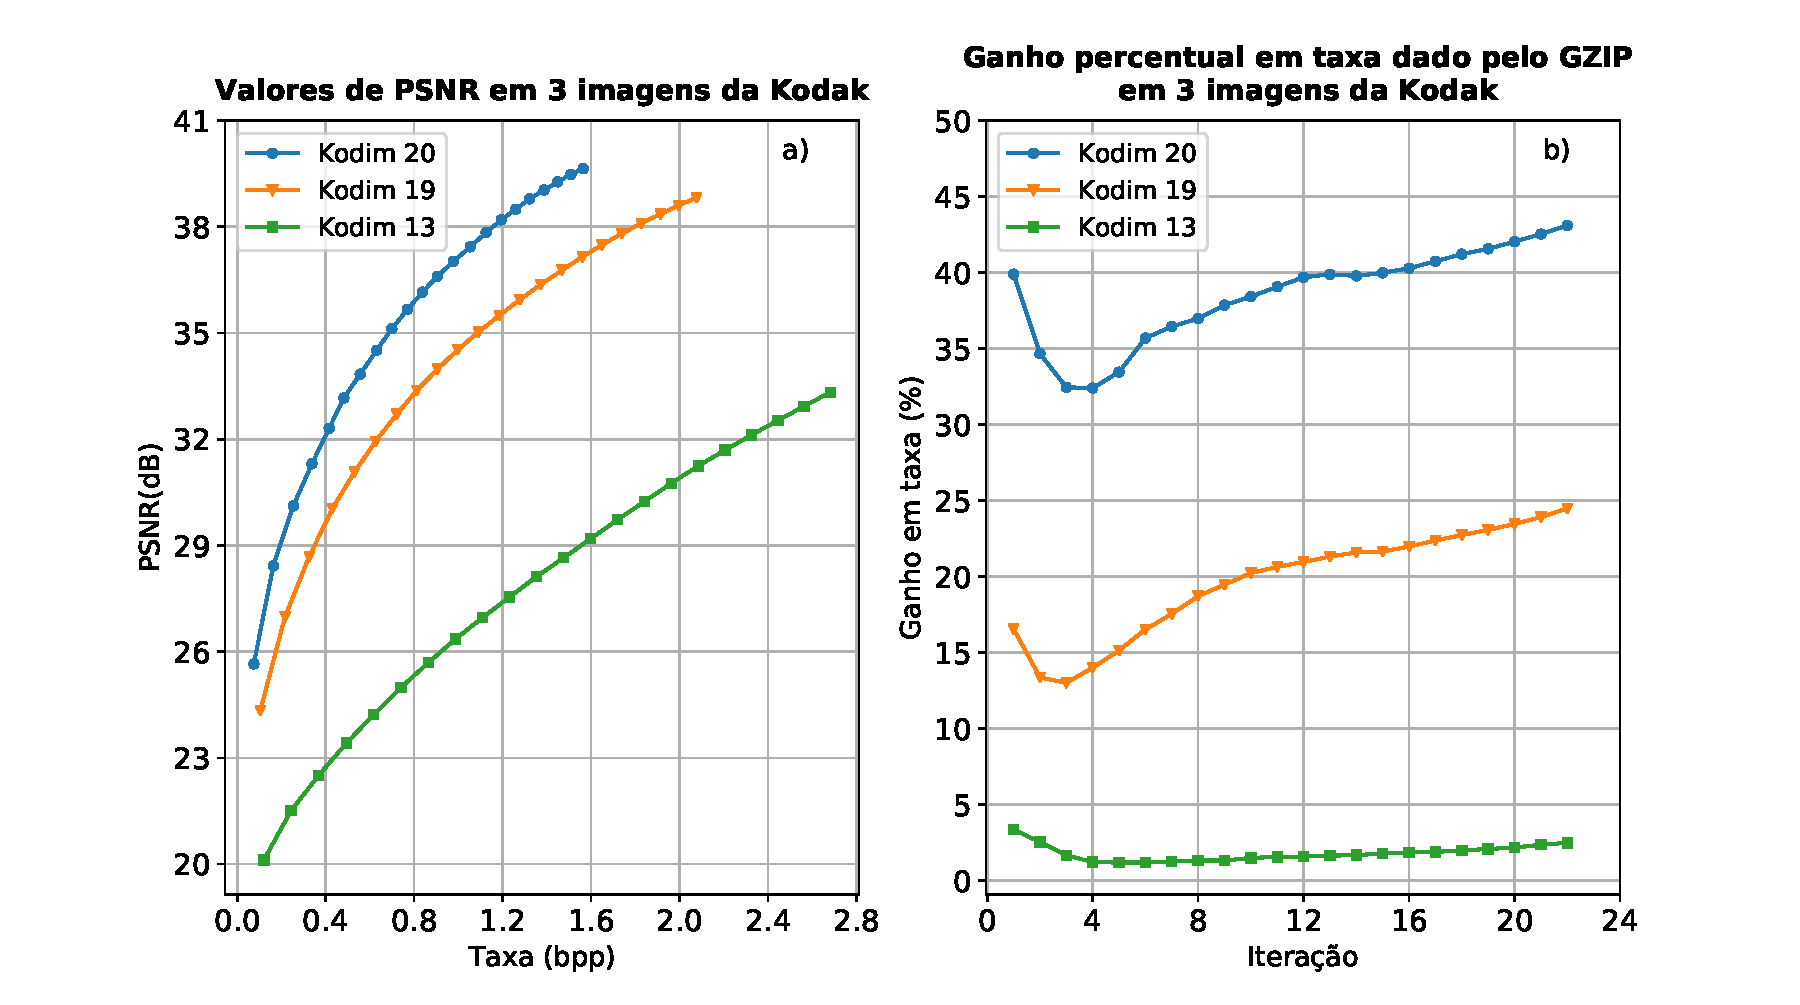
\includegraphics[width=1.0\textwidth]{figuras/comp_gain_psnr.pdf}
	\caption{}  	
	\label{fig:comp_gain_psnr}
\end{figure}

%	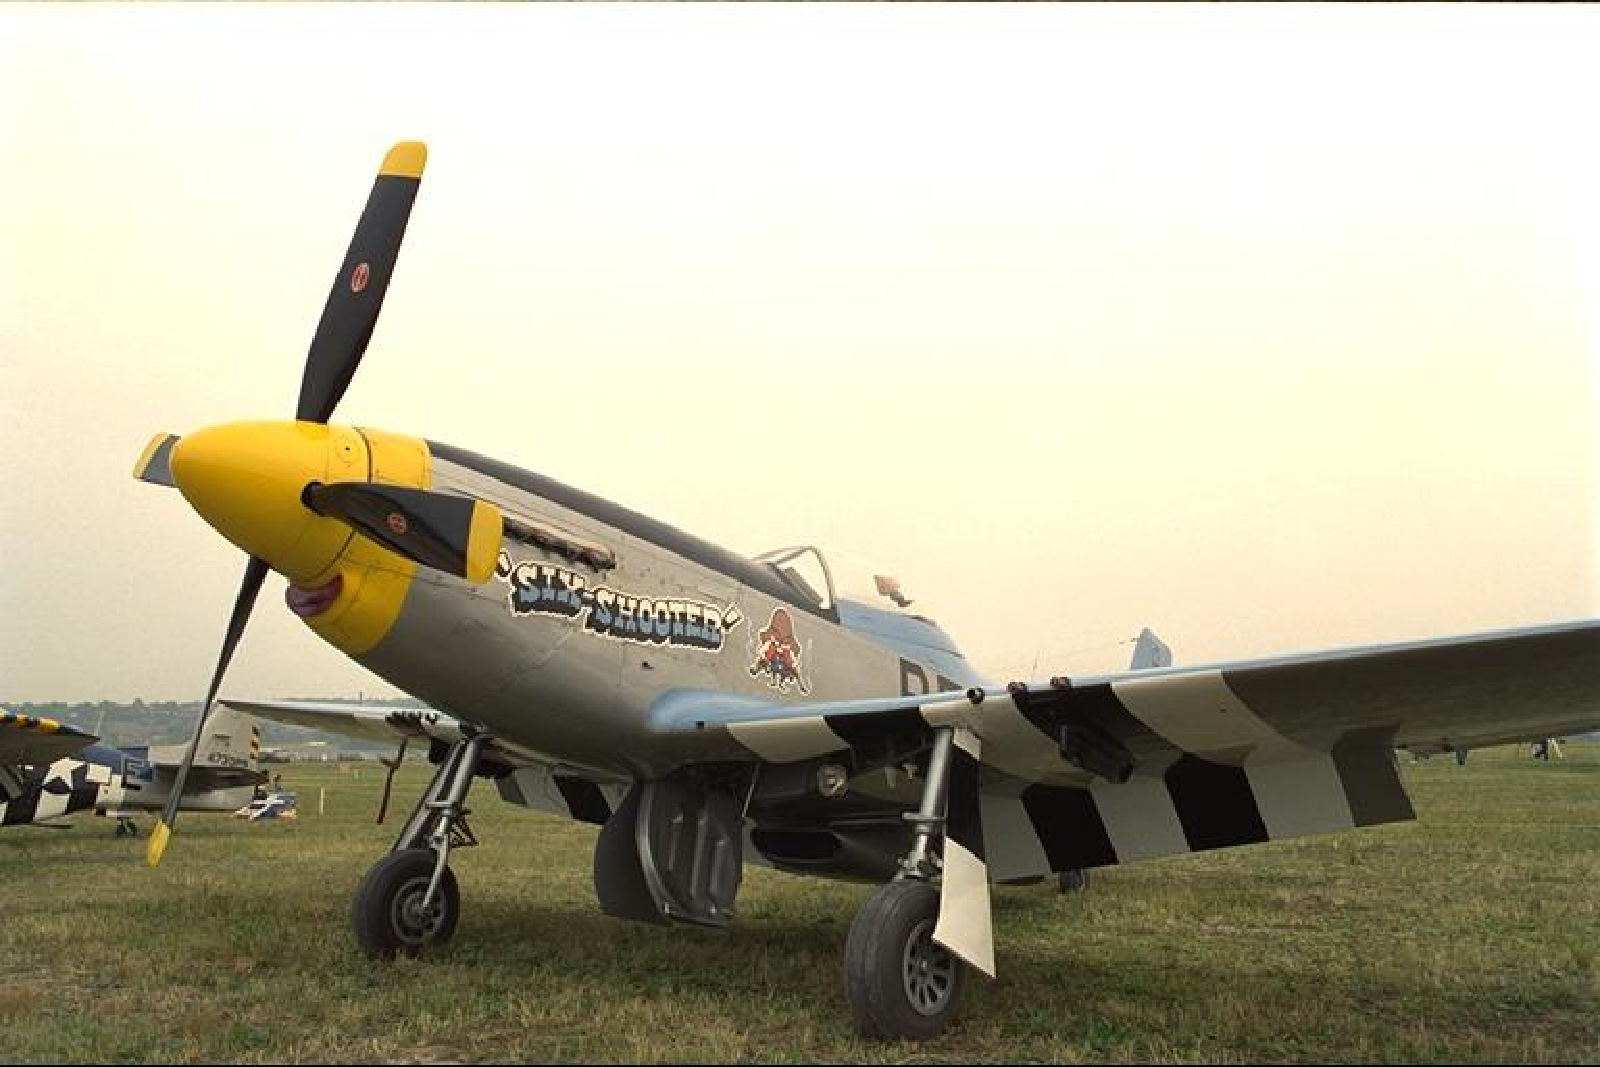
\includegraphics[width=.4\linewidth]{figuras/kodim20}



\begin{figure}
	
	\subfloat[Imagem original]{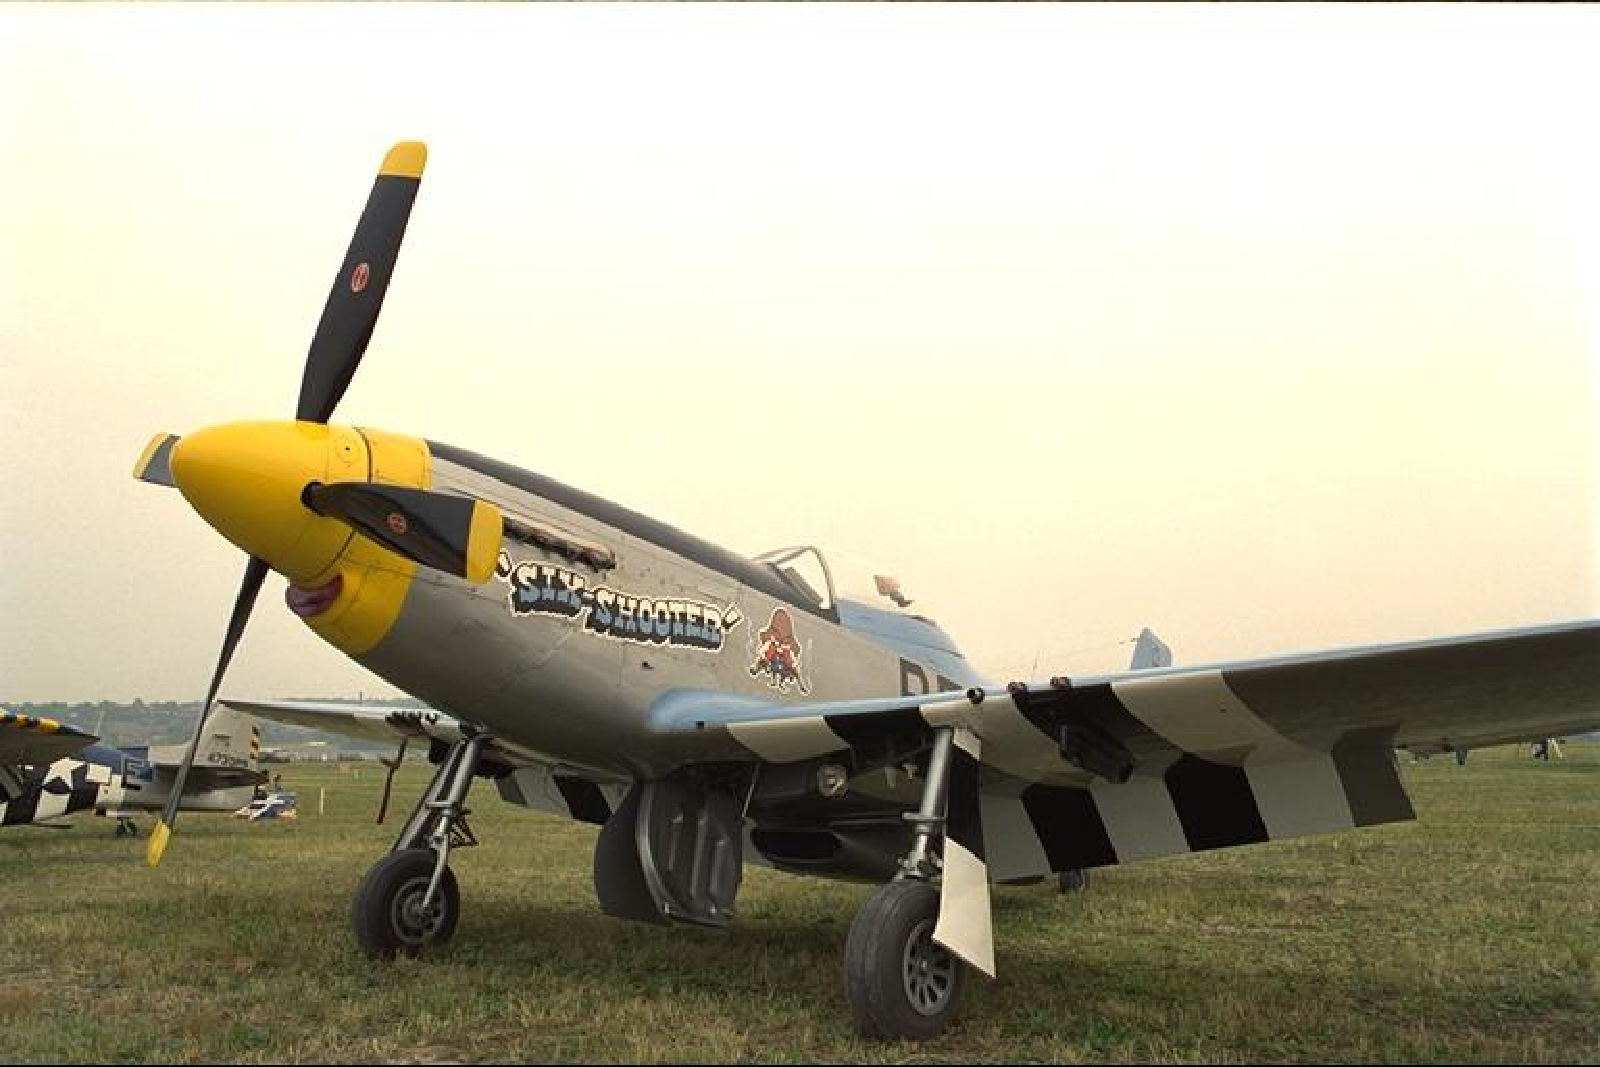
\includegraphics[width=0.45\textwidth]{figuras/kodim20.pdf}}
	\hfill
	\subfloat[{Imagem reconstruída. Taxa: 0,942 bpp. PSNR: 36,925 dB.}   ]{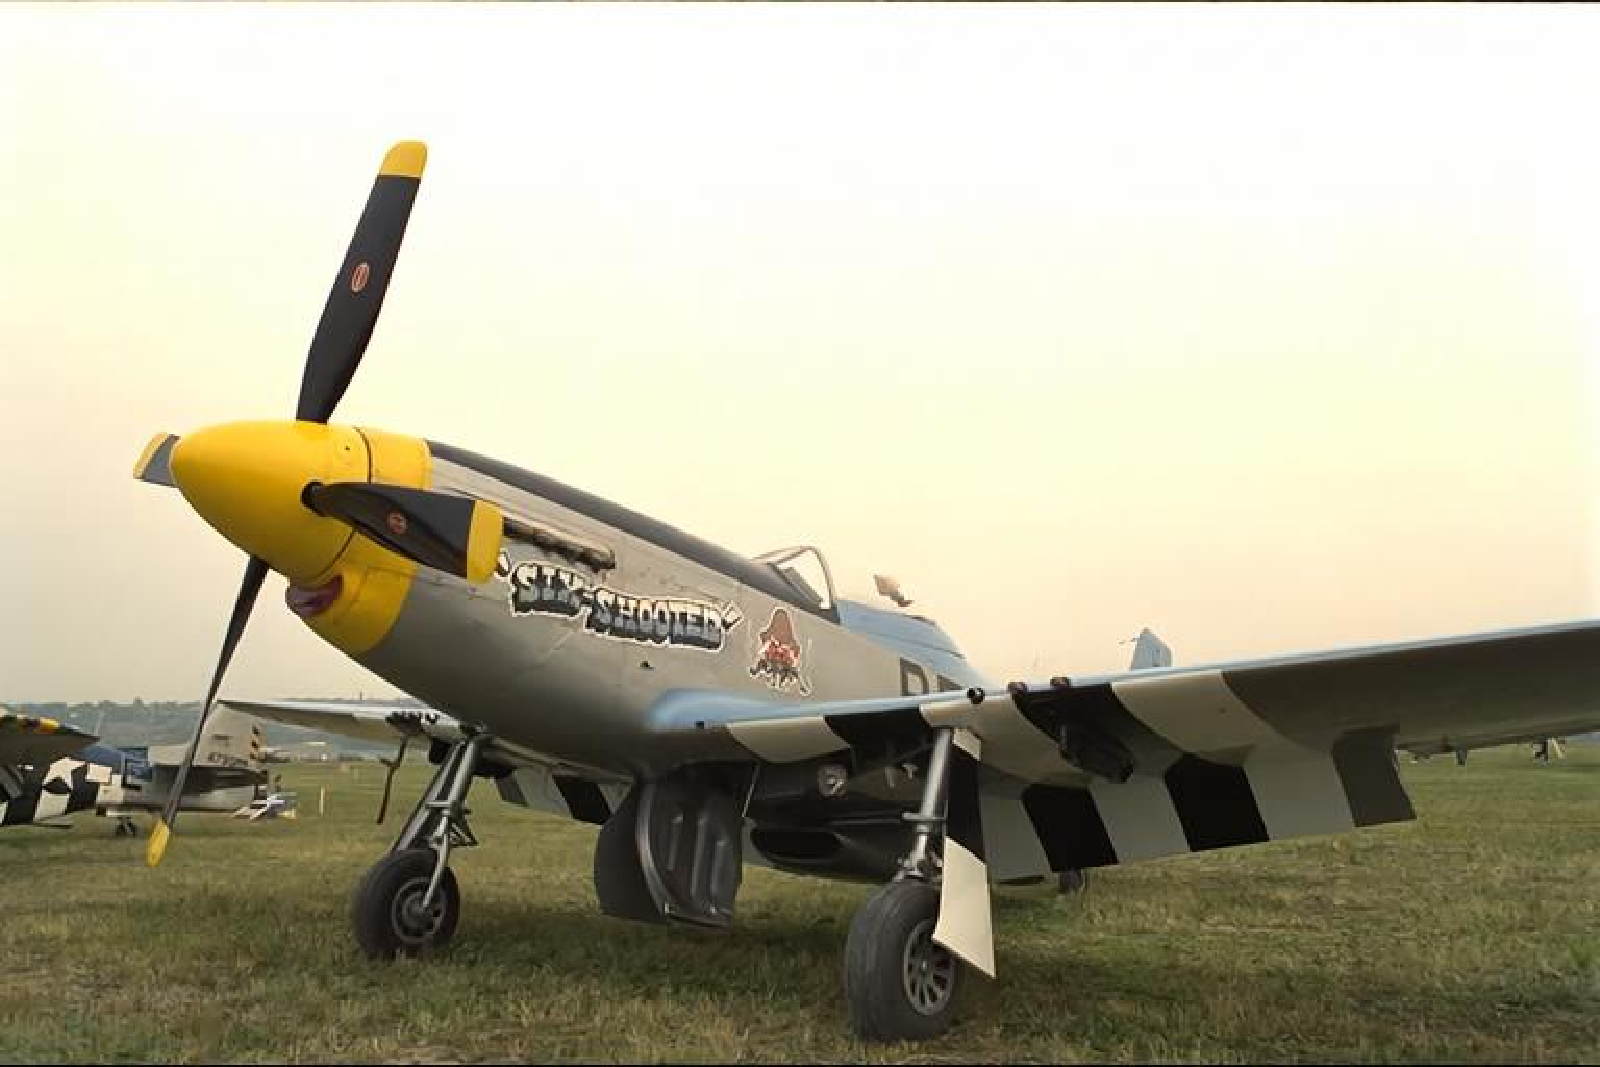
\includegraphics[width=0.45\textwidth]{figuras/kodim20it10.pdf}}
	
	\subfloat[Imagem original]{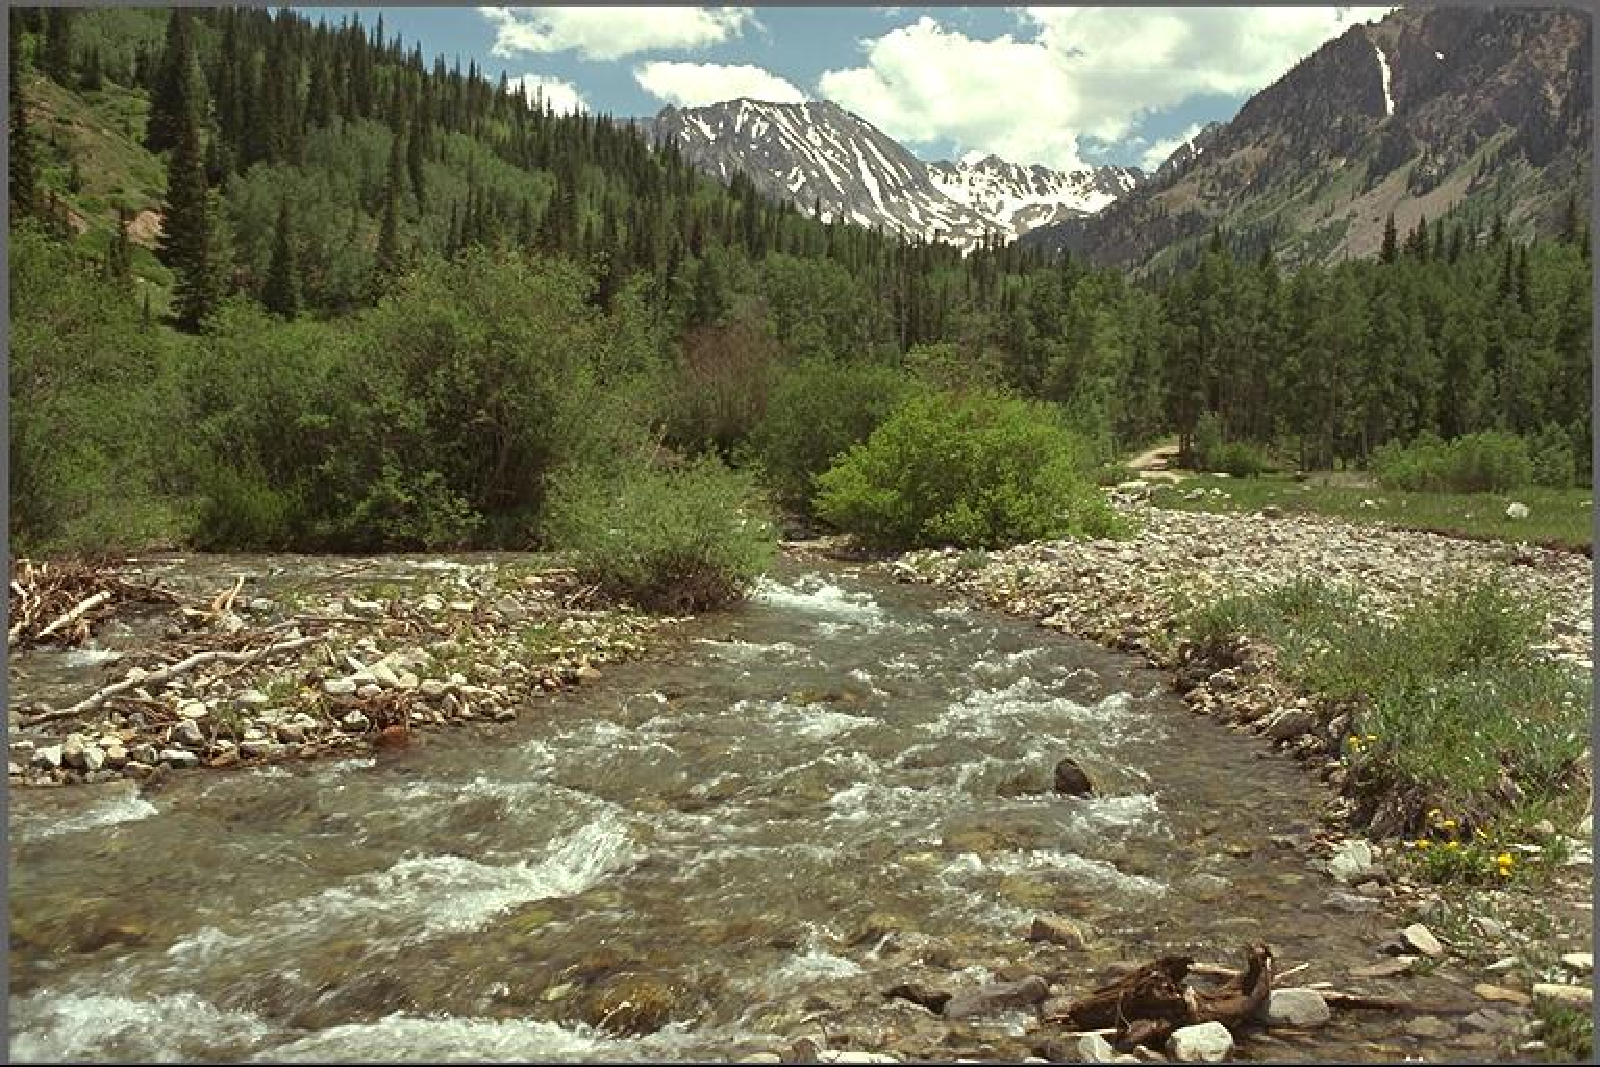
\includegraphics[width=0.45\textwidth]{figuras/kodim13.pdf}}
	\hfill
	\subfloat[{Imagem reconstruída. Taxa: 0,987 bpp. PSNR: 26,357 dB.}   ]{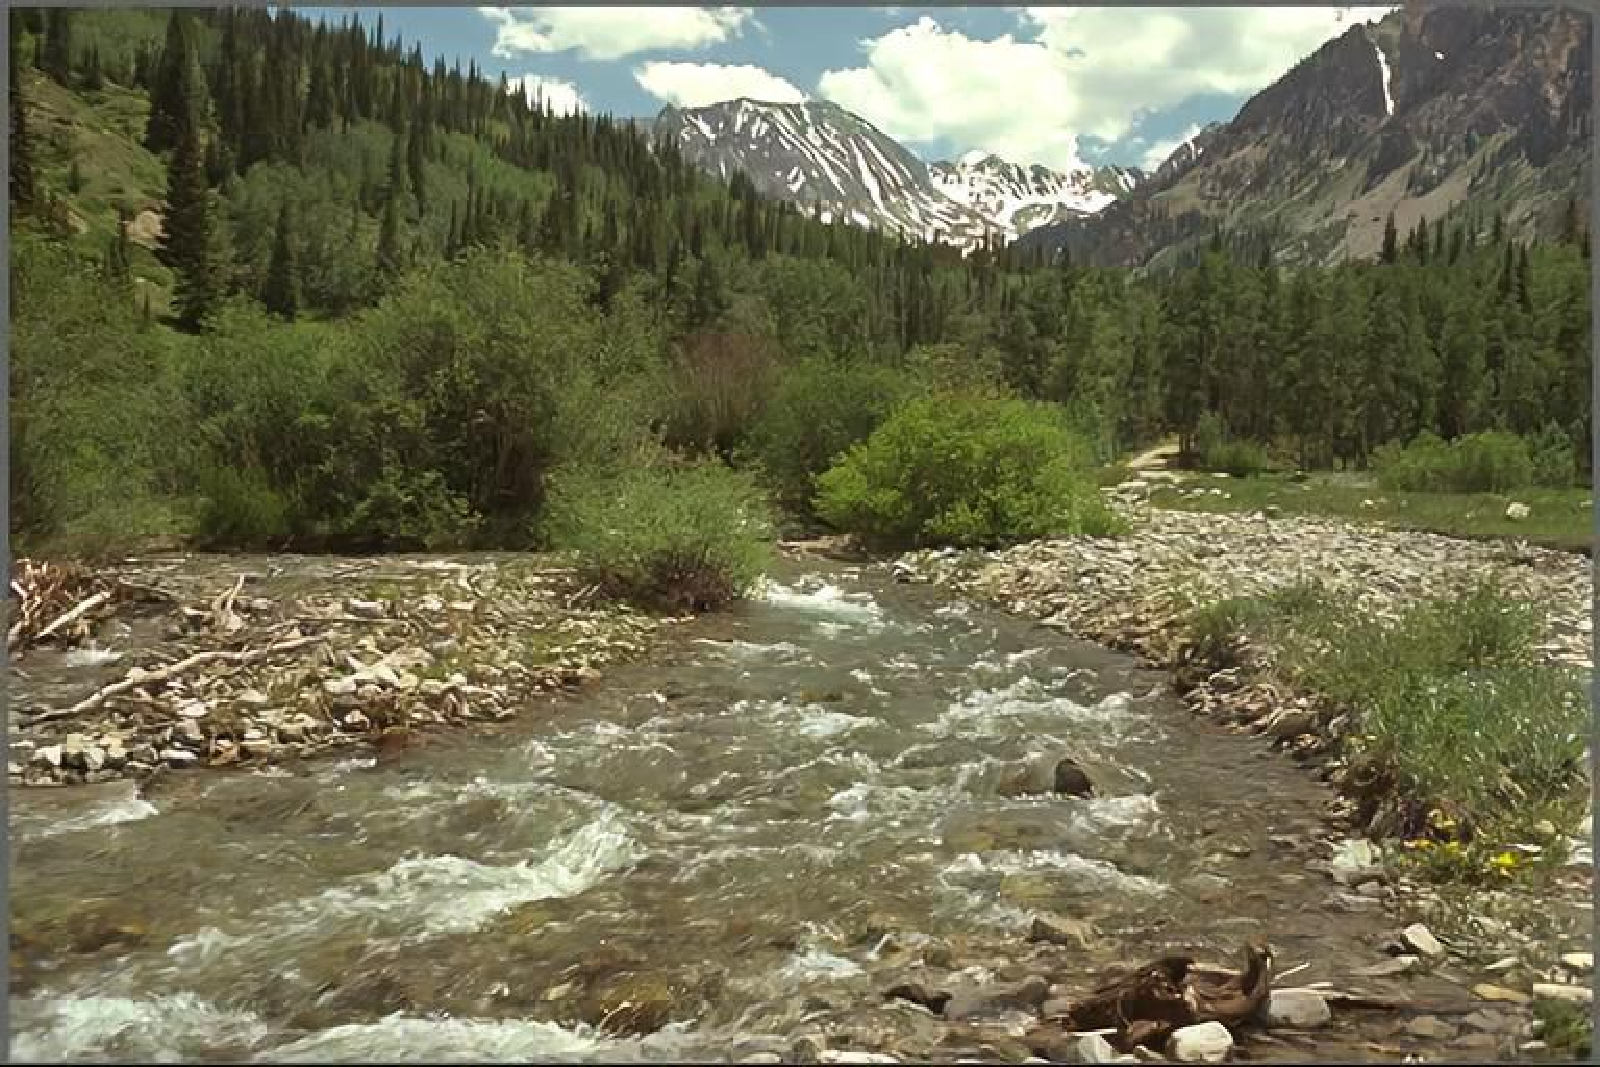
\includegraphics[width=0.45\textwidth]{figuras/kodim13it8.pdf}}
	\caption{Em (a) temos a Kodim10 original em (b) sua versão reconstruída em 10 iterações. Em (c) está representado a kodim13 e em (d) sua sua reconstruída em 8 iterações.}
	\label{fig:kodim13}
\end{figure}
No método de alocação dinâmica de bits descrito em \ref{sec:adb} fizemos dois testes principais. No primeiro, não havia restrição do mínimo de níveis de reconstrução ou iterações em cada bloco, isso equivale a fazer $k_min=1$ em \ref{fig:flux_vr}. Vamos no referir a ele como modeloVR0. Contudo, tal procedimento gera artefatos de blocos em evidência, como podemos observar na Figura \ref{fig:artf}. Então, fazemos $k_min=1$ para codificar as imagens pelo modeloVR e tentar minimizar o surgimento desses artefatos de compressão.   
No exemplo apresentado na Figura \ref{fig:artf]}

\begin{figure}
	
	\subfloat[Imagem original]{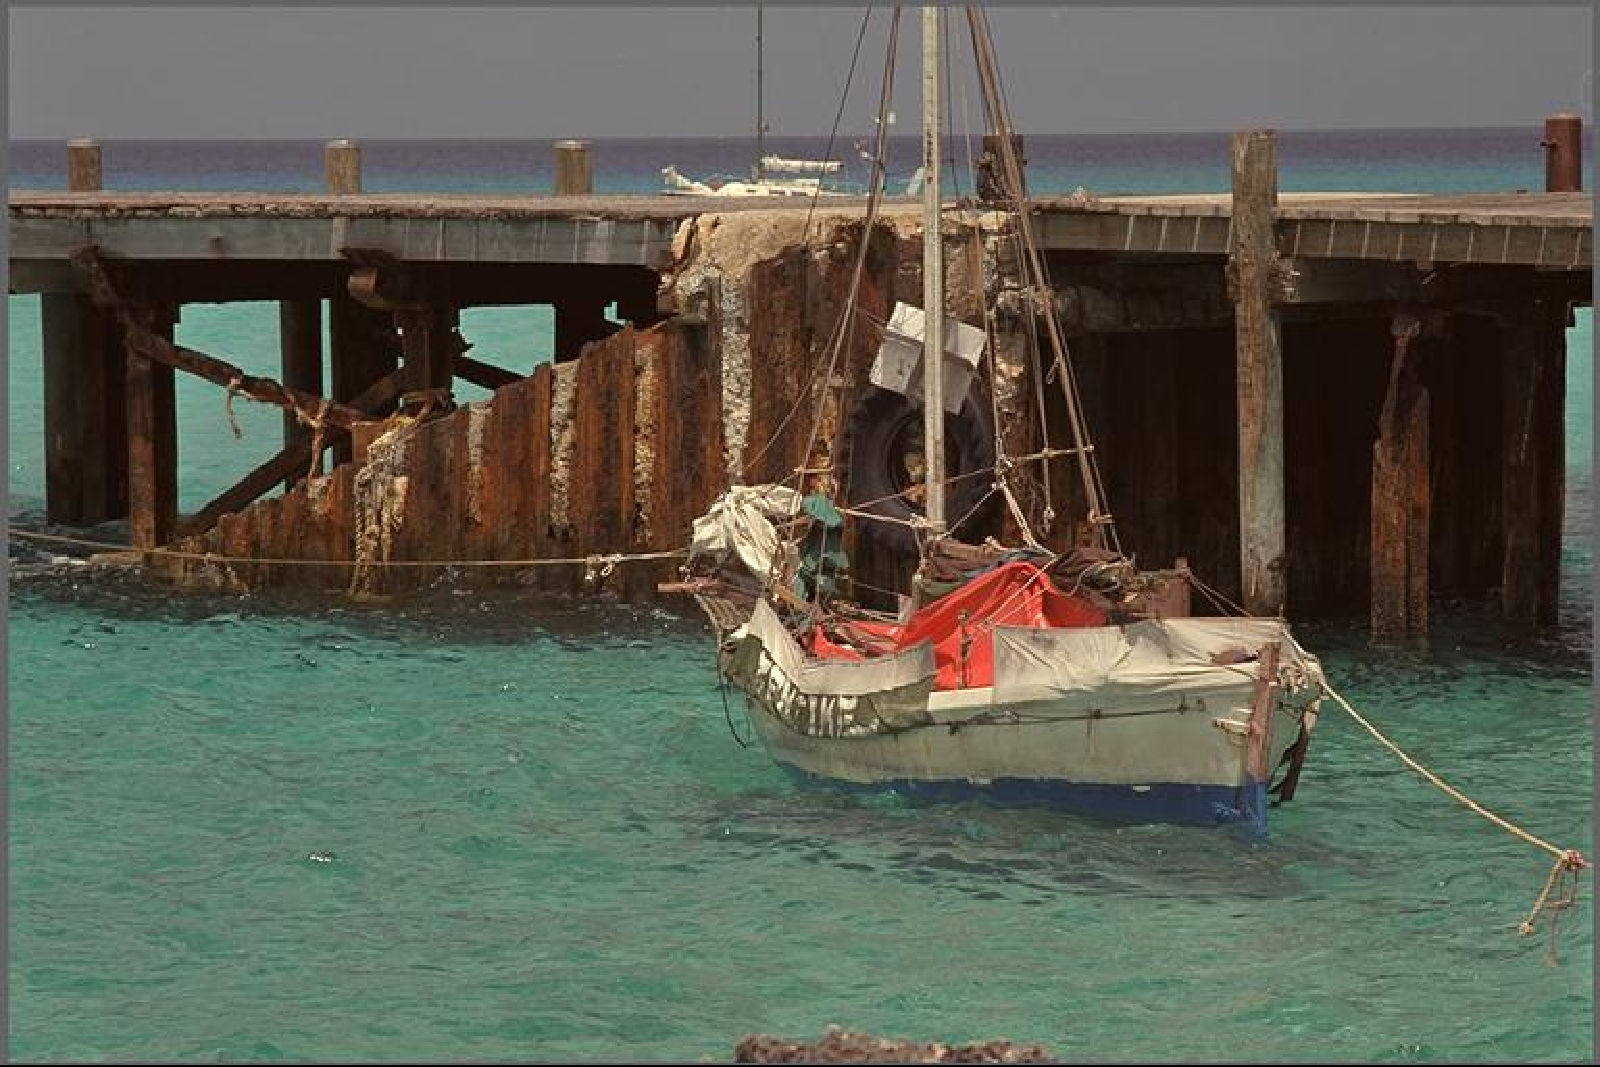
\includegraphics[width=0.45\textwidth]{figuras/kodim11.pdf}}
	\hfill
	\subfloat[{Imagem reconstruída. Taxa: 0,741 bpp, PSNR: 32,190dB, SSIM: 0,8675.}   ]{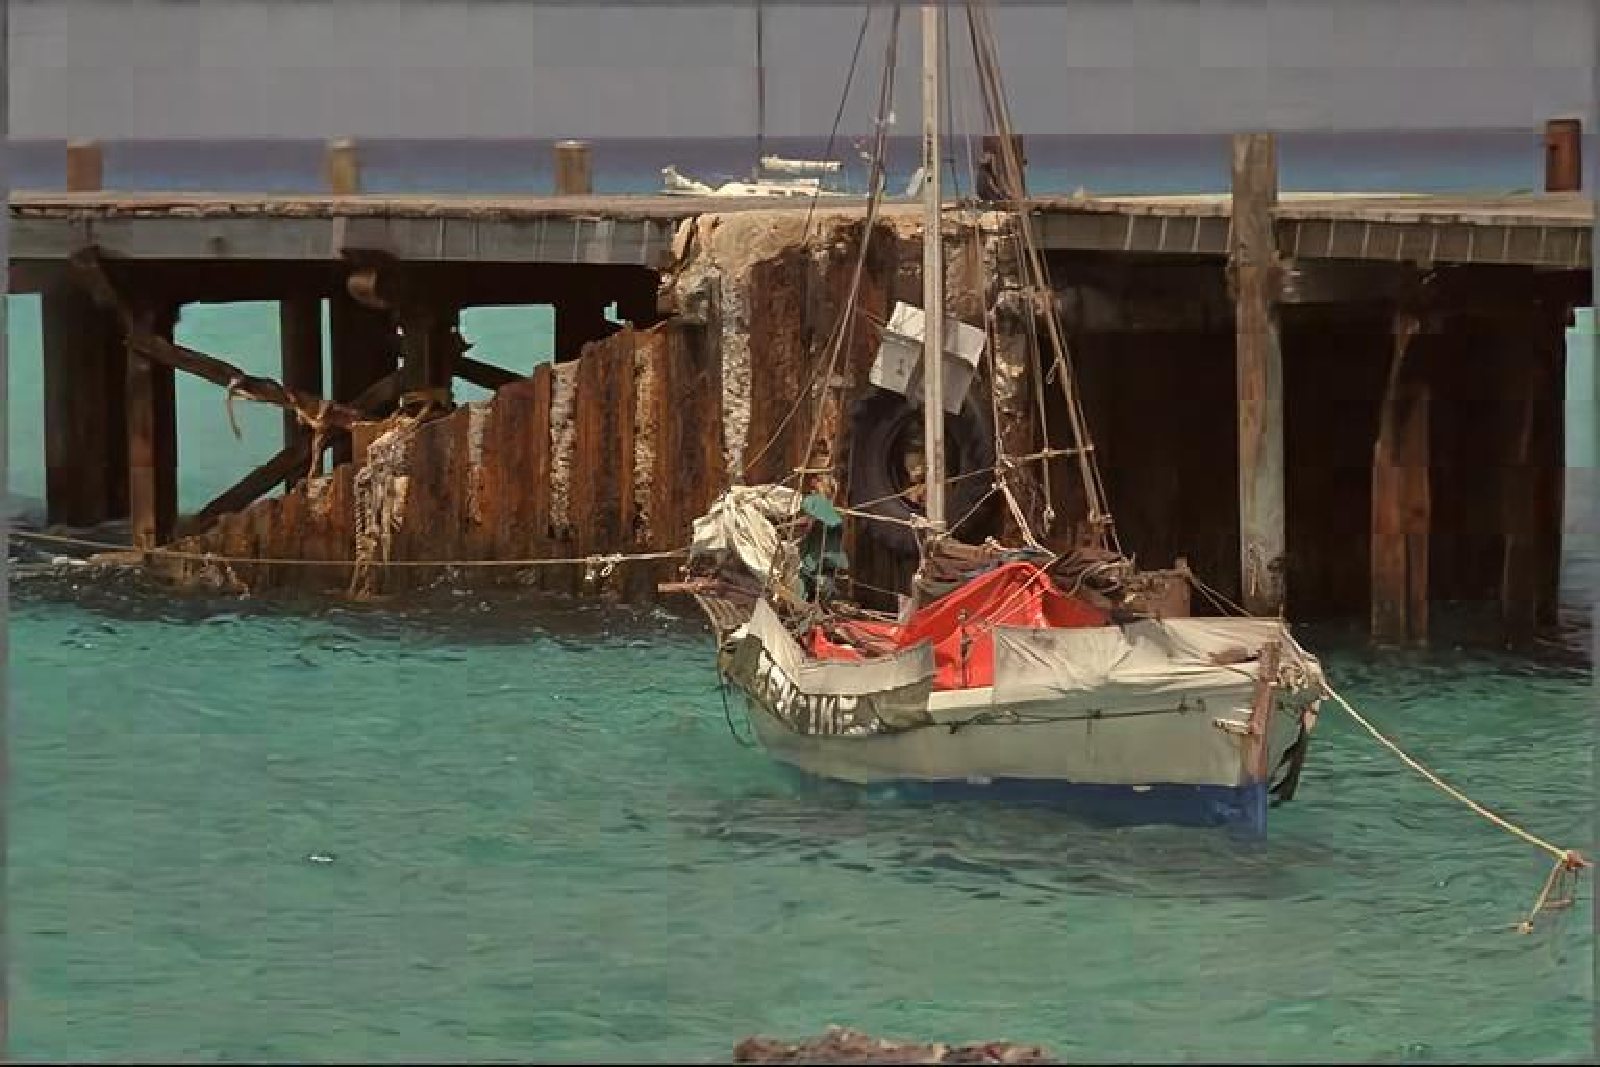
\includegraphics[width=0.45\textwidth]{figuras/kodim11targ_1_2431.pdf}}
	
	\subfloat[Imagem reconstruída. Taxa: 0,782 bpp, PSNR: 32,687dB, SSIM: 0,8939]{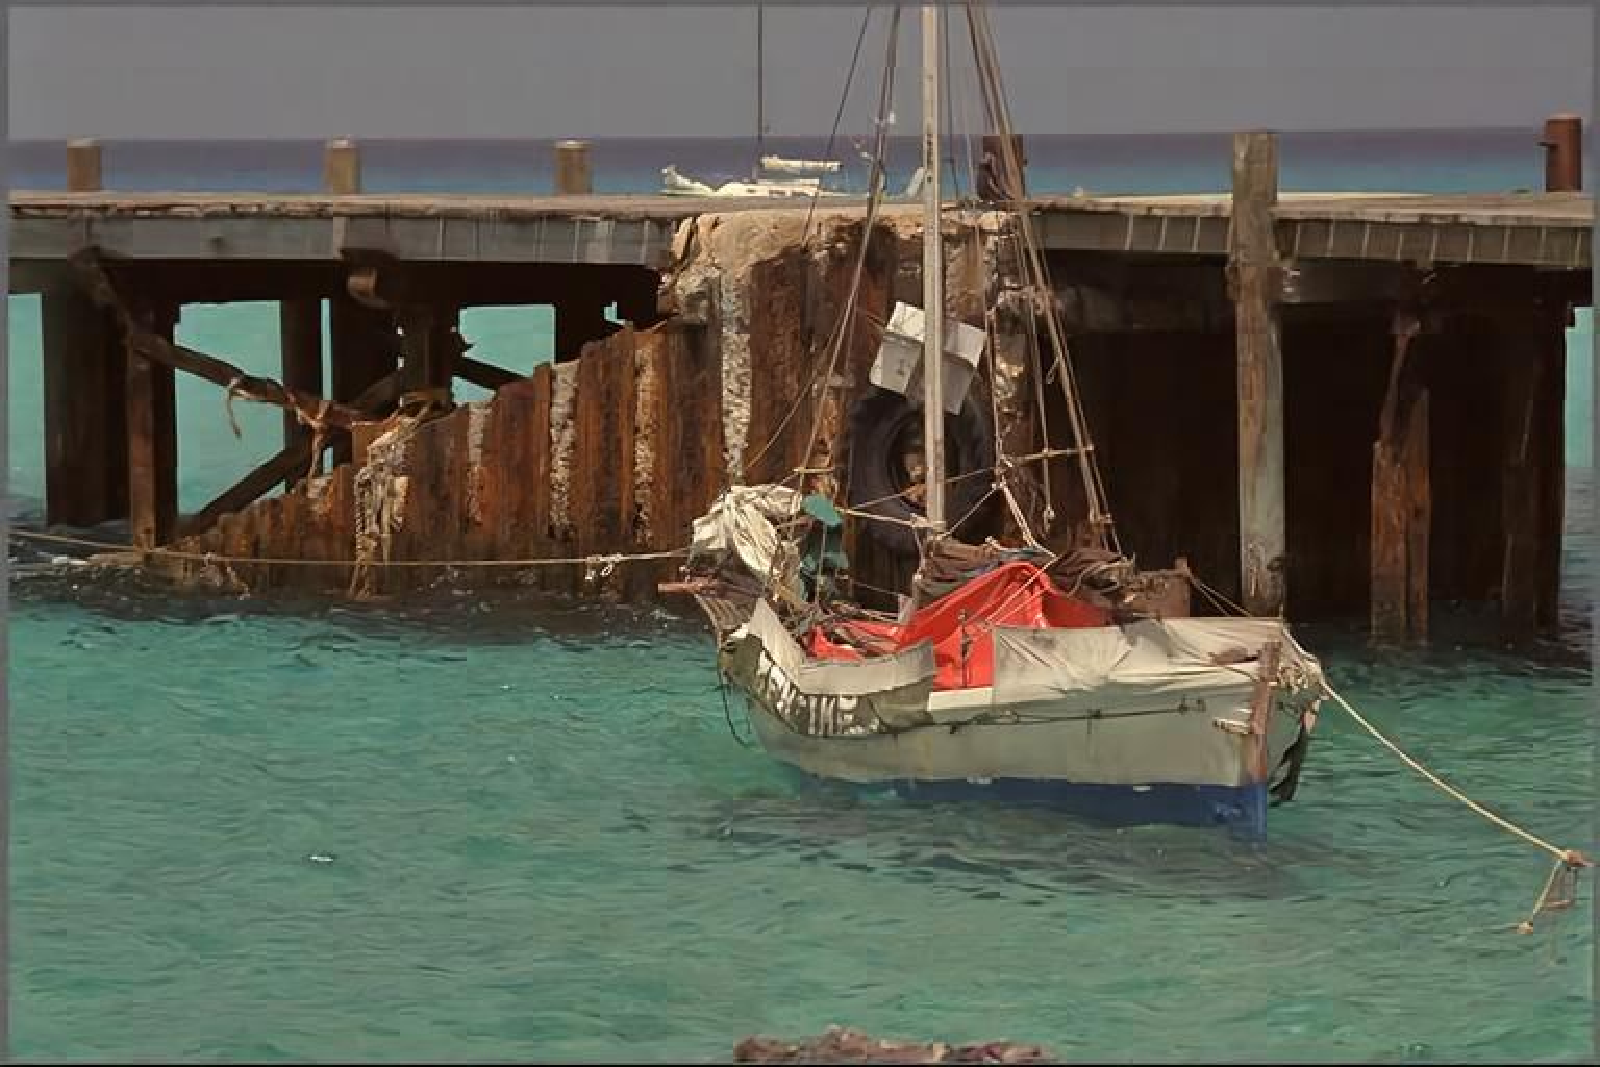
\includegraphics[width=0.45\textwidth]{figuras/kodim11targ30.pdf}}
	\hfill
	\subfloat[{Imagem reconstruída. Taxa: 0,754 bpp, PSNR: 31,621, SSIM:0,8985 }   ]{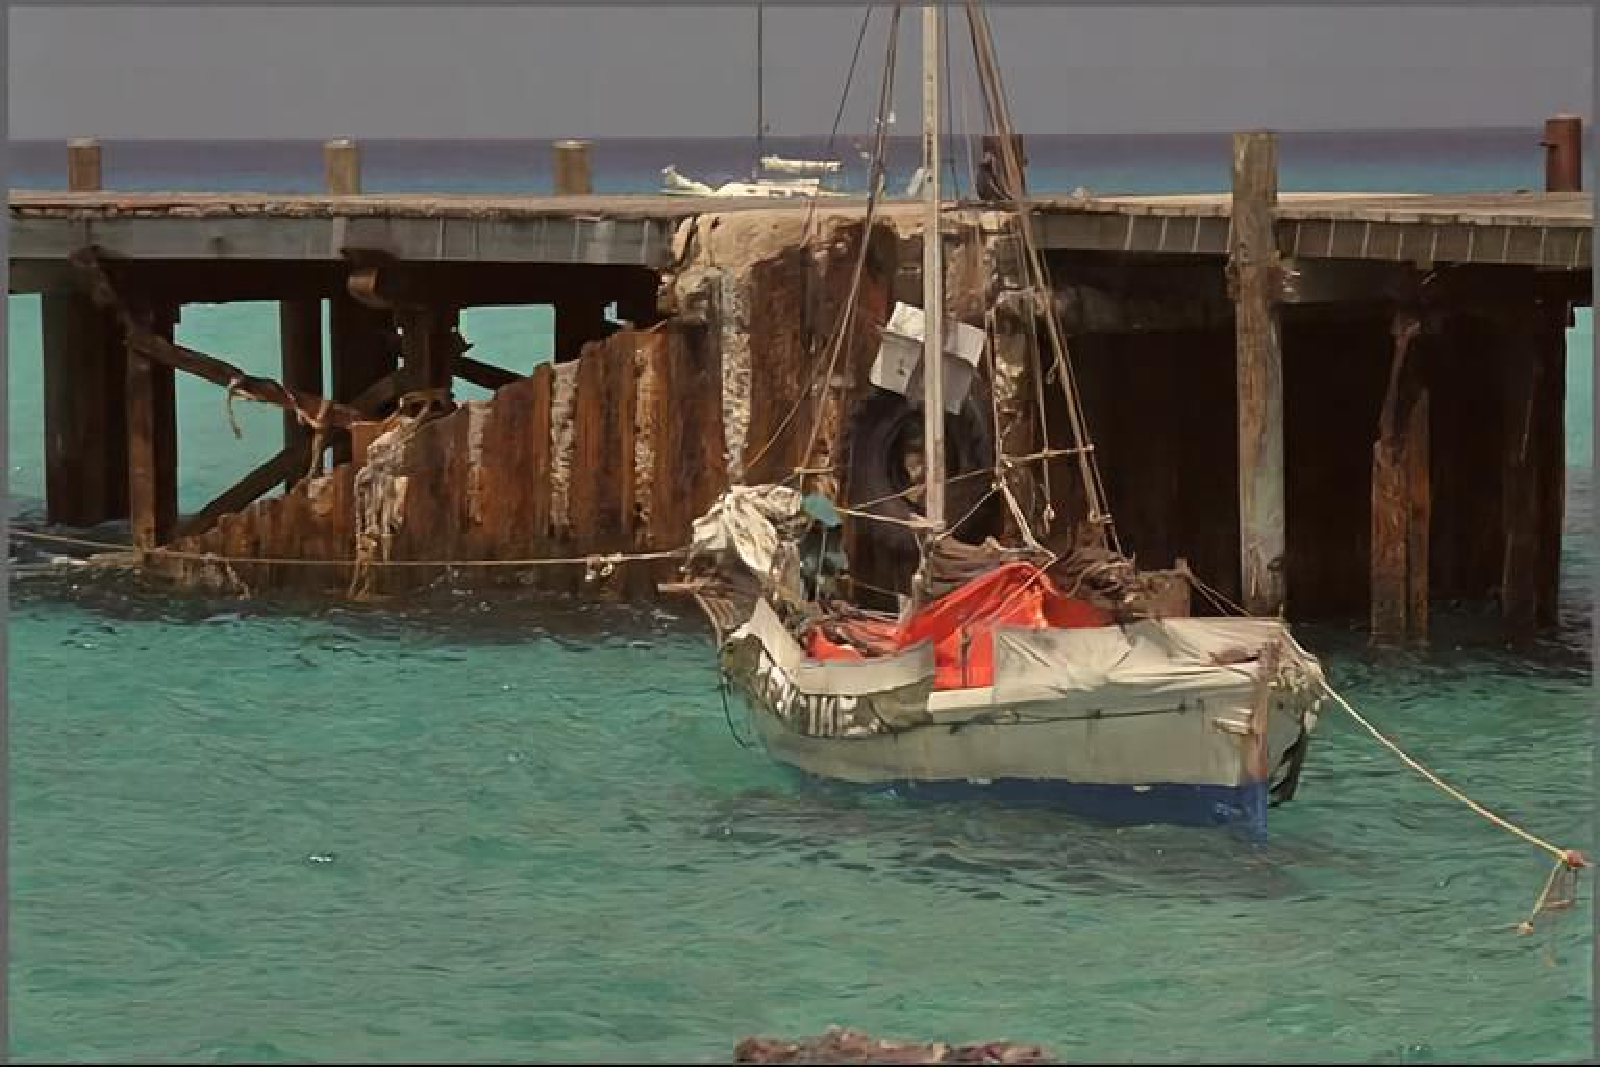
\includegraphics[width=0.45\textwidth]{figuras/kodim11it7.pdf}}
	\label{fig:artf}
	\caption[Surgimento de artefatos de blocos em modelos baseados em alocação de bits.]{Em (a) temos a kodim11 original. A figura (b) é uma reconstrução com o modeloVR0. Em (c) a imagem é codificada pelo modeloVR de alocação de bits. Por fim, em (d) é sua reconstrução com o modelo26 usando 7 níveis de resíduo.}
	
\end{figure}

A Figura \ref{fig:comp_vr}

\begin{figure}
	\centering
	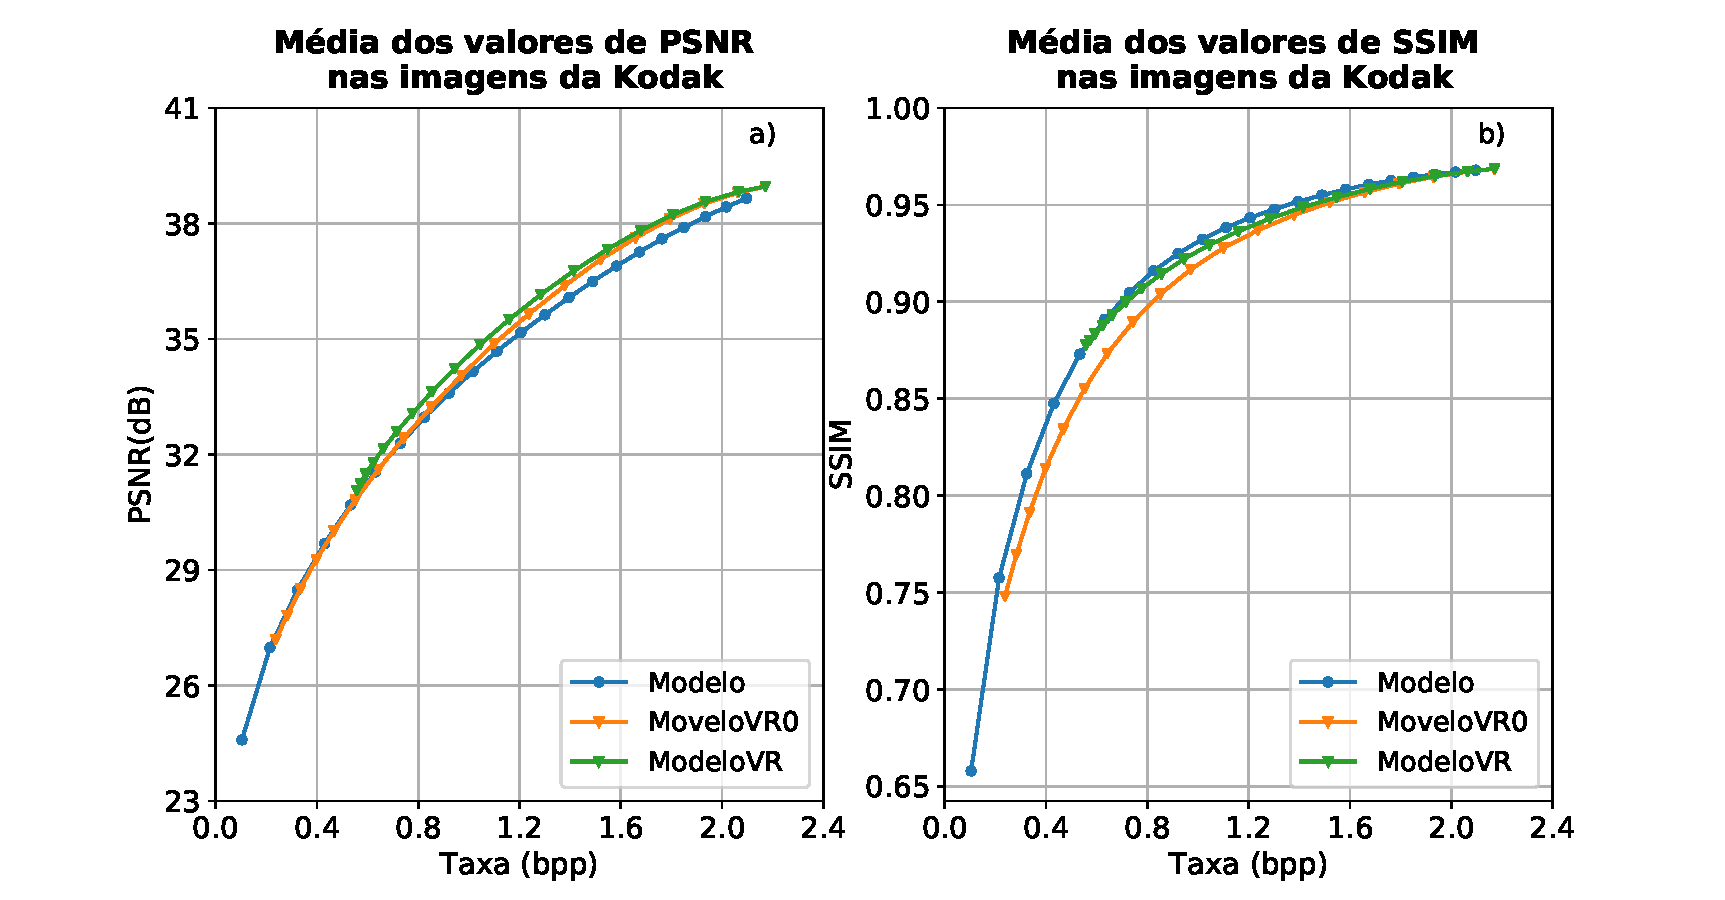
\includegraphics[width=1.0\textwidth]{figuras/com_vr.pdf}
	\caption{}  	
	\label{fig:comp_vr}
\end{figure}

\begin{figure}
	\centering
	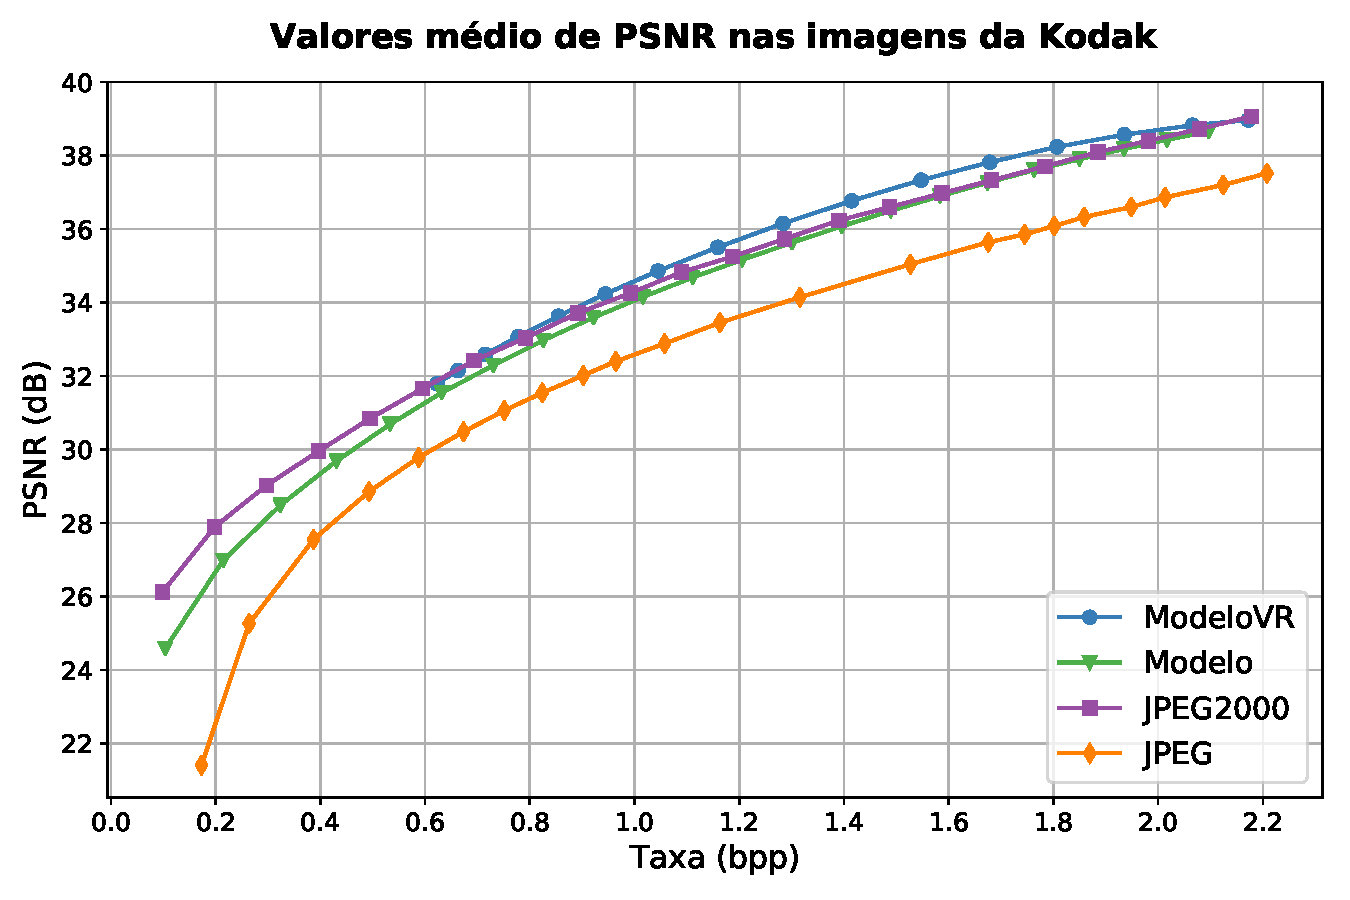
\includegraphics[width=1.0\textwidth]{figuras/comp_codecs.pdf}
	\caption{}  	
	\label{fig:comp_codecs}
\end{figure}
